%%% TeX-command-extra-options: "-shell-escape"
% \documentclass{llncs}
\documentclass[a4paper,UKenglish,cleveref, autoref, thm-restate]{lipics-v2021}
% \documentclass[llncs, a4paper, UKenglish, cleveref, autoref, thm-restate]{article}
\usepackage[utf8]{inputenc} % Required for inputting international characters
\usepackage[T1]{fontenc} % Output font encoding for international characters
% \usepackage[backend=bibtex,style=alphabetic,natbib=true]{biblatex}
% \usepackage[backend=bibtex,style=alphabetic,natbib=true]{biblatex}
% \addbibresource{references.bib}

\usepackage{amsmath, mathpartir, stmaryrd}
%, amssymb, amsfonts, stmaryrd}
% \usepackage{mathpartir}
% \usepackage{bussproofs}

\usepackage{caption}
\usepackage{subcaption}
\usepackage{graphicx}
\usepackage{enumitem}
\usepackage{xparse}
\usepackage[usenames, dvipsnames]{xcolor}
\usepackage{lipsum}
\usepackage{xargs}
\usepackage{hyperref}
\usepackage{tikz-cd}
\usepackage{todonotes}
\usepackage{url}
\usepackage{xspace}
\usepackage{rotating}
\usepackage{quiver}
\usepackage{minted}
\usepackage{newunicodechar}
\usepackage{microtype}
% \addbibresource{references.bib}
\usepackage{array}   % for \newcolumntype macro
\newcolumntype{C}{>{$}c<{$}} % math-mode version of "l" column type
\newcolumntype{L}{>{$}l<{$}} % math-mode version of "l" column type

\usepackage{inconsolata}
% \usepackage{draftwatermark}
% \SetWatermarkText{Confidential}
% \SetWatermarkScale{4}
% \SetWatermarkColor[gray]{0.9}

\hypersetup{
  linktocpage,
  colorlinks,
  citecolor=BlueViolet,
  filecolor=red,
  linkcolor=Blue,
  urlcolor=BrickRed
}
\newcommand{\mpav}[1]{\textcolor{red}{\textsc{Marco}: #1}}
\newcommand{\dcas}[1]{\textcolor{ForestGreen}{\textsc{David}: #1}}
\newcommand{\mvol}[1]{\textcolor{blue}{\textsc{Michael}: #1}}
% \newcommand{\proofcomment}[1]{\text{\{ #1 \}}}
% \newenvironment{proofof}[1] {\begin{proof}[Proof of {#1}]}{\end{proof}}
\newcommand{\eqdef}{\stackrel{\mathrm{\Delta}}{=}}
\newcommand{\eqiff}{\stackrel{\triangle}{\iff}}
\newcommand{\bnfeq}{\mathrel{::=}}
\newcommand{\defeq}{\triangleq}
\newcommand{\rul}[3]{\frac{#2}{#3}\;  {\textrulelabel{#1}}}
\newcommand{\den}[1]{\llbracket #1 \rrbracket}
\newcommand{\jud}[3]{#1 \vdash #2 : #3}
\newcommand{\bden}[1]{\llparenthesis#1 \rrparenthesis}
\newcommand{\bigslant}[2]{{\raisebox{.2em}{$#1$}\left/\raisebox{-.2em}{$#2$}\right.}}
\newcommand{\quotient}[2]{\bigslant{#1}{#2}}
\newcommand{\curry}{\Lambda}
\newcommand{\uncurry}{\begin{sideways}\begin{sideways}$\Lambda$\end{sideways}\end{sideways}}
\newcommand{\Bool}{\mathbb{B}}
\newcommand{\N}{\mathbb{N}}
\newcommand{\Nat}{\N}
\newcommand{\R}{\mathbb{R}}
\newcommand{\Sets}{\mathbf{Set}}
\newcommand{\blacklater}{\blacktriangleright}
\newcommand{\tot}{\mathcal{S}}
\newcommand{\PSh}{\ensuremath{\textbf{PSh}(\omega)}}

\newsavebox{\lbananabox}
\newcommand{\lbananamacro}{%
  
\begin{tikzpicture}[baseline=0.25em,xscale=0.005em,yscale=0.005em]
  \draw[solid, join=round] (2,0) to[out=140,in=-90] (0,3) to[out=90,in=-140] (2,6) -- (2.1,5.9)
              to[out=-120,in=90] (1.2,3) to[out=-90,in=120] (2.1,0.1) -- cycle;
\end{tikzpicture}
}
\savebox{\lbananabox}{\lbananamacro}
\newcommand{\lbanana}{\mathopen{\usebox{\lbananabox}\hspace{-0.6ex}}}


\newsavebox{\rbananabox}
\newcommand{\rbananamacro}{%
  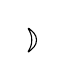
\begin{tikzpicture}[baseline=0.25em,xscale=-0.005em,yscale=0.005em]
  \draw[solid, join=round] (2,0) to[out=140,in=-90] (0,3) to[out=90,in=-140] (2,6) -- (2.1,5.9)
              to[out=-120,in=90] (1.2,3) to[out=-90,in=120] (2.1,0.1) -- cycle;
  \end{tikzpicture}
}
\savebox{\rbananabox}{\rbananamacro}
\newcommand{\rbanana}{\mathclose{\usebox{\rbananabox}}}


\newsavebox{\lbansbox}
\newcommand{\lbansmacro}{%
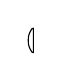
\begin{tikzpicture}[baseline=0.45ex,xscale=0.006em,yscale=0.012ex]%
% curvey bananas
%\draw[solid,join=round,fill=yellow] (2,0) to[out=140,in=-90] (0,3) to[out=90,in=-140] (2,6) -- (2.1,5.9) to[out=-120,in=90] (1.2,3) to[out=-90,in=120] (2.1,0.1) -- cycle;%
% fitted lenses
\draw[solid,join=round] (1.8,6) -- (1.5,5.9) to[out=-120, in=90] (0.7,3) to[out=-90, in=120] (1.5,0.1) -- (1.8,0) -- cycle;%
\end{tikzpicture}}
\savebox{\lbansbox}{\lbansmacro}
\newcommand{\lbans}{\mathopen{\usebox{\lbansbox}\mspace{1mu}}}

\newsavebox{\rbansbox}
\newcommand{\rbansmacro}{%
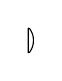
\begin{tikzpicture}[baseline=0.45ex,xscale=-0.006em,yscale=0.012ex]%
% curvey bananas
%\draw[solid,join=round,fill=yellow] (2,0) to[out=140,in=-90] (0,3) to[out=90,in=-140] (2,6) -- (2.1,5.9) to[out=-120,in=90] (1.2,3) to[out=-90,in=120] (2.1,0.1) -- cycle;%
% fitted lenses
\draw[solid,join=round] (1.8,6) -- (1.5,5.9) to[out=-120, in=90] (0.7,3) to[out=-90, in=120] (1.5,0.1) -- (1.8,0) -- cycle;%
\end{tikzpicture}}
\savebox{\rbansbox}{\rbansmacro}
\newcommand{\rbans}{\mathclose{\mspace{1mu}\usebox{\rbansbox}}}

\newsavebox{\llensbox}
\newcommand{\llensmacro}{%
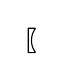
\begin{tikzpicture}[baseline=0.45ex,xscale=0.006em,yscale=0.012ex]%
\draw[solid,join=round] (1.4,0) -- (0,0) -- (0,6) -- (1.4,6) -- (1.5,5.9) to[out=-120, in=90] (0.7,3) to[out=-90, in=120] (1.5,0.1) -- cycle;%
\end{tikzpicture}}
\savebox{\llensbox}{\llensmacro}
\newcommand{\llens}{\mathopen{\usebox{\llensbox}\mspace{1mu}}}

\newsavebox{\rlensbox}
\newcommand{\rlensmacro}{%
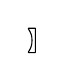
\begin{tikzpicture}[baseline=0.45ex,xscale=-0.006em,yscale=0.012ex]%
\draw[solid,join=round] (1.4,0) -- (0,0) -- (0,6) -- (1.4,6) -- (1.5,5.9) to[out=-120, in=90] (0.7,3) to[out=-90, in=120] (1.5,0.1) -- cycle;%
\end{tikzpicture}}
\savebox{\rlensbox}{\rlensmacro}
\newcommand{\rlens}{\mathclose{\mspace{1mu}\usebox{\rlensbox}}}

% filled versions
\newcommand{\Lbanana}{%
  \mathopen{\mspace{1mu}\tikz[baseline=0.25em,xscale=0.006em,yscale=0.006em]
  \fill (2,0) to[out=140,in=-90] (0,3) to[out=90,in=-140] (2,6) -- (2.1,5.9)
              to[out=-120,in=90] (1.2,3) to[out=-90,in=120] (2.1,0.1) -- cycle;\mspace{1mu}}}
\newcommand{\Rbanana}{%
  \mathclose{\mspace{1mu}\tikz[baseline=0.25em,xscale=-0.006em,yscale=0.006em]
  \fill (2,0) to[out=140,in=-90] (0,3) to[out=90,in=-140] (2,6) -- (2.1,5.9)
              to[out=-120,in=90] (1.2,3) to[out=-90,in=120] (2.1,0.1) -- cycle;}}
% % lens brackets (using TikZ)
% \newcommand{\llens}{%
%   \mathopen{\tikz[baseline=0.25em,xscale=0.006em,yscale=0.006em]
%   \draw[join=round] (1.4,0) -- (0,0) -- (0,6) -- (1.4,6) -- (1.5,5.9)
%         to[out=-120,in=90] (0.7,3) to[out=-90,in=120] (1.5,0.1) -- cycle;\mspace{1mu}}}
% \newcommand{\rlens}{%
%   \mathclose{\mspace{1mu}\tikz[baseline=0.25em,xscale=-0.006em,yscale=0.006em]
%   \draw[join=round] (1.4,0) -- (0,0) -- (0,6) -- (1.4,6) -- (1.5,5.9)
%         to[out=-120,in=90] (0.7,3) to[out=-90,in=120] (1.5,0.1) -- cycle;}}
% filled versions
\newcommand{\Llens}{%
  \mathopen{\tikz[baseline=0.25em,xscale=0.006em,yscale=0.006em]
  \fill (1.4,0) -- (0,0) -- (0,6) -- (1.4,6) -- (1.5,5.9)
        to[out=-120,in=90] (0.7,3) to[out=-90,in=120] (1.5,0.1) -- cycle;\mspace{1mu}}}
\newcommand{\Rlens}{%
  \mathclose{\mspace{1mu}\tikz[baseline=0.25em,xscale=-0.006em,yscale=0.006em]
  \fill (1.4,0) -- (0,0) -- (0,6) -- (1.4,6) -- (1.5,5.9)
        to[out=-120,in=90] (0.7,3) to[out=-90,in=120] (1.5,0.1) -- cycle;}}


\newcommand{\anamor}[1]{{\llens\, #1\, \rlens}}
\newcommand{\catamor}[1]{\lbanana\, #1\, \rbanana}
\newcommand{\cata}[1]{\catamor{#1}}
\newcommand{\ana}[1]{\llens #1 \rlens}
\newcommand{\catafree}[1]{\Lbanana #1 \Rbanana}
\newcommand{\anacofree}[1]{\Llens #1 \Rlens}
\newcommand{\hylo}[2]{\cata{#1 \to #2}}
\newcommand{\cohylo}[2]{\ana{#1 \to #2}}
\newcommand{\fold}[1]{\catamor{#1}}
\newcommand{\unfold}[1]{\anamor{#1}}
\newcommand{\comp}{\cdot}
\newcommand{\operator}[1]{\textsf{#1}}
\newcommand{\head}{\operator{head}}
\newcommand{\inl}{\operator{inl}}
\newcommand{\inr}{\operator{inr}}
\newcommand{\tail}{\operator{tail}}
\newcommand{\Alg}{\text{-Alg}}
\newcommand{\Coalg}{\text{-CoAlg}}
\newcommand{\Free}{\text{Free\xspace}}
\newcommand{\fmap}[1]{\text{fmap}\;#1}

\newcommand{\zero}{\operator{zero}}
\newcommand{\Nil}{\operator{nil}}
\newcommand{\Succ}{\operator{succ}}

\newcommand{\InOp}{\operator{in}^{\circ}}
\newcommand{\InIso}{\operator{in}}
\newcommand{\OutOp}{\operator{out}^{\circ}}
\newcommand{\OutIso}{\operator{out}}
\newcommand{\call}{\operator{call}}

\newcommand{\CatC}{\mathcal{C}}
\newcommand{\CatD}{\mathcal{D}}
\newcommand{\CatE}{\mathcal{E}}
\newcommand{\CatI}{\mathcal{I}}
\newcommand{\Set}{\mathbf{Set}}
\newcommand{\Type}{\mathbf{Type}}
\newcommand{\iso}{\cong}
\newcommand{\ceiling}[1]{\lceil #1 \rceil}
\newcommand{\floor}[1]{\lfloor #1 \rfloor}
\newcommand{\pair}[2]{\langle #1, #2 \rangle}
\newcommand{\haskell}[1]{\mintinline{haskell}{#1}}
%\newcommand{\coq}[1]{\mintinline{coq}{#1}}

\newcommand{\Hom}{\text{Hom}}
\newcommand{\Obj}{\text{Obj}}
\newcommand{\Arr}{\text{Arr}}

\newcommand{\Str}[1]{\operator{Str}(#1)}
\newcommand{\List}[1]{\operator{List}(#1)}
\newcommand{\Strbare}{\operator{Str}}
\newcommand{\Listbare}{\operator{List}}
\newcommand{\nil}{\operator{nil}}
\newcommand{\cons}{\operator{cons}}
\newcommand{\foldr}{\operator{foldr}}

\newcommand{\vcomp}{\circ}

\newmintinline[coq]{coq}{fontsize=\small, breaklines}
\newmintinline[ocaml]{OCaml}{fontsize=\small}
\newminted{coq}{fontsize=\small}
\newminted{ocaml}{fontsize=\small}

\title{Program Optimisations via Hylomorphisms for Extraction of Executable Code}

\bibliographystyle{plainurl}% the mandatory bibstyle
%\titlerunning{Dummy short title} %TODO optional, please use if title is longer than one line

%%%%%%%%%%%%%%%%%%%%%%%%%%%%%%%%%%%%%%%%%%%%%%%%%%%%%%%%%%%%%%%%%%%%%%%%%%%
% LNCS author information
% \author{David Castro Perez\inst{1}\orcidID{0000-0002-6939-4189} \and
% Marco Paviotti\inst{2,3}\orcidID{0000-0002-1513-0807} \and
% Michael Vollmer\inst{3}\orcidID{0000-0002-0496-8268}}
% %
% \authorrunning{D. Castro Perez et al.}
% % First names are abbreviated in the running head.
% % If there are more than two authors, 'et al.' is used.
% %
% \institute{University Of Kent, Canterbury, CT2 7NZ, United Kingdom\\
% \email{\{D.Castro-Perez, M.Paviotti, M.Vollmer\}@kent.ac.uk}}
%%%%%%%%%%%%%%%%%%%%%%%%%%%%%%%%%%%%%%%%%%%%%%%%%%%%%%%%%%%%%%%%%%%%%%%%%%%


%%%%%%%%%%%%%%%%%%%%%%%%%%%%%%%%%%%%%%%%%%%%%%%%%%%%%%%%%%%%%%%%%%%%%%%%%%%
% LIPICS author information
\author{David {Castro Perez}}%
{University Of Kent, Canterbury, CT2 7NZ, United Kingdom}%
{D.Castro-Perez@kent.ac.uk}%
{0000-0002-6939-4189}%
{EP/Y00339X/1, EP/T014512/1}
\author{Marco Paviotti}%
{University Of Kent, Canterbury, CT2 7NZ, United Kingdom}%
{M.Paviotti@kent.ac.uk}%
{0000-0002-1513-0807}%
{}
\author{Michael Vollmer}%
{University Of Kent, Canterbury, CT2 7NZ, United Kingdom}%
{M.Vollmer@kent.ac.uk}%
{0000-0002-0496-8268}%
{}

\authorrunning{D. Castro Perez et al.}
%%%%%%%%%%%%%%%%%%%%%%%%%%%%%%%%%%%%%%%%%%%%%%%%%%%%%%%%%%%%%%%%%%%%%%%%%%%

% \author{Jane {Open Access}}{Dummy University Computing Laboratory, [optional: Address], Country \and My second affiliation, Country \and \url{http://www.myhomepage.edu} }{johnqpublic@dummyuni.org}{https://orcid.org/0000-0002-1825-0097}{(Optional) author-specific funding acknowledgements}%TODO mandatory, please use full name; only 1 author per \author macro; first two parameters are mandatory, other parameters can be empty. Please provide at least the name of the affiliation and the country. The full address is optional. Use additional curly braces to indicate the correct name splitting when the last name consists of multiple name parts.

% \author{Joan R. Public\footnote{Optional footnote, e.g. to mark corresponding author}}{Department of Informatics, Dummy College, [optional: Address], Country}{joanrpublic@dummycollege.org}{[orcid]}{[funding]}

\Copyright{Jane Open Access and Joan R. Public} %TODO mandatory, please use full first names. LIPIcs license is "CC-BY";  http://creativecommons.org/licenses/by/3.0/

% \ccsdesc[100]{\textcolor{red}{Replace ccsdesc macro with valid one}} %TODO mandatory: Please choose ACM 2012 classifications from https://dl.acm.org/ccs/ccs_flat.cfm

\begin{CCSXML}
<ccs2012>
   <concept>
       <concept_id>10003752.10010124.10010125.10010127</concept_id>
       <concept_desc>Theory of computation~Functional constructs</concept_desc>
       <concept_significance>500</concept_significance>
       </concept>
   <concept>
       <concept_id>10003752.10003790.10011740</concept_id>
       <concept_desc>Theory of computation~Type theory</concept_desc>
       <concept_significance>300</concept_significance>
       </concept>
   <concept>
       <concept_id>10003752.10010124.10010138.10010142</concept_id>
       <concept_desc>Theory of computation~Program verification</concept_desc>
       <concept_significance>500</concept_significance>
       </concept>
 </ccs2012>
\end{CCSXML}

\ccsdesc[500]{Theory of computation~Functional constructs}
\ccsdesc[300]{Theory of computation~Type theory}
\ccsdesc[500]{Theory of computation~Program verification}

\keywords{hylomorphisms, program calculation, divide and conquer, fusion} %TODO mandatory; please add comma-separated list of keywords

\category{} %optional, e.g. invited paper

% \acknowledgements{I want to thank \dots}
% optional

%\nolinenumbers %uncomment to disable line numbering

%Editor-only macros:: begin (do not touch as author)%%%%%%%%%%%%%%%%%%%%%%%%%%%%%%%%%%
\EventEditors{}
\EventNoEds{2}
\EventLongTitle{ITP 2025)}
\EventShortTitle{ITP 2025}
\EventAcronym{ITP}
\EventYear{2025}
\EventDate{December 24--27, 2016}
\EventLocation{Little Whinging, United Kingdom}
\EventLogo{}
\SeriesVolume{42}
\ArticleNo{23}
%%%%%%%%%%%%%%%%%%%%%%%%%%%%%%%%%%%%%%%%%%%%%%%%%%%%%%

\begin{document}

\maketitle

%TODO mandatory: add short abstract of the document
\begin{abstract}
  Generic programming with recursion schemes provides a powerful abstraction for
  structuring recursion and provides a rigorous reasoning principle for program
  optimisations which have been successfully applied to compilers for functional
  languages. Formalising recursion schemes in a type theory offers additional
  termination guarantees, but it often requires compromising on performance,
  requiring the assumption of additional axioms, and/or introducing unsafe casts
  into extracted code.

  This paper presents the first Rocq formalisation of \emph{hylomorphisms}
  allowing for the mechanisation of all recognised recursive algorithms. The key
  contribution of this paper is that this formalisation is fully
  \emph{axiom-free}, and it allows the extraction of safe, idiomatic functional
  code. We exemplify the framework by formalising a series of algorithms based
  on different recursive paradigms such as divide-and conquer, dynamic
  programming, and mutual recursion and demonstrate that the extracted
  functional code for the programs formalised in our framework is efficient,
  humanly readable, and runnable. Furthermore, we show the use of the
  machine-checked proofs of the laws of hylomorphisms to do program
  optimisations.
\end{abstract}

\section{Introduction}
\label{sec:intro}
Over the years, extensive research has been conducted on program calculation
techniques, a well-established approach for deriving efficient programs from
simpler specifications through systematic program
transformation~\cite{gibbonsSquiggol, BirddeMoor96:Algebra}. A key aspect of
this approach is the use of structured recursion schemes, which serve as
powerful abstractions that capture common patterns of recursion. By structuring
computation in this way, programs benefit from well-established \emph{algebraic
properties} that provide a solid foundation for reasoning about program
equivalences, transformations, and optimisations -- such as \emph{fusion} laws or
semi-automatic parallelisations~\cite{TakanoM95,Gibbons96:Third,Morihata09:Third,farmsCastro}.
In the context of \emph{program calculation}, these algebraic properties allow
programmers to describe code using simple, inefficient specifications within an
\emph{algebra of programming}~\cite{BirddeMoor96:Algebra}. They can then apply
algebraic laws to systematically \emph{calculate} more efficient versions of the
same algorithms.

Suppose, for example, that we want to write a program that sorts a list of
integers and multiplies them by 2 at the same time. In OCaml, we may write this
function directly:

\pagebreak
\begin{minted}{ocaml}
let rec sort_times_two = function
  | [] -> []
  | h :: t -> let (l, r) = partition (fun x -> x < h) t in
  sort_times_two l @ (h * 2) :: sort_times_two r
\end{minted}

This program is the same as composing a \emph{quicksort} OCaml implementation,
with the function \ocaml{map (fun x -> x * 2)} which is a known program
optimisation called \emph{fusion}.  A lot of program calculations have this
pattern: start from a simple specification, e.g.
\\$\mathsf{map}\;(\lambda x.\;x \times 2) \circ \mathsf{sort}$, and use program
equivalences and algebraic laws to rewrite it to an optimised version. We will
revisit a similar example in Section~\ref{sec:sorting}.

This program calculation stems from the more general theory of hylomorphisms. A
hylomorphism is a structured recursion scheme representing the idea of a
divide-and-conquer algorithm where, first, the problem is split into smaller
sub-problems (divide), then sub-solutions are computed recursively, and,
finally, these sub-solutions are put together to compute the solution to the
original problem (conquer). This general pattern of recursion induces a
reasoning principle, called the \emph{fusion law}, which has been exemplified in
the previous paragraph. By leveraging this principle, we can systematically
transform recursive definitions into more efficient versions while preserving
correctness.
% This program calculation stems from the more general theory of hylomorphisms.  A
% hylomorphism is a structured recursion scheme representing the idea of a
% divide-and-conquer algorithm where, first, the problem is split into smaller
% sub-problems (divide), then sub-solutions are computed recursively, and, finally,
% these sub-solutions are put together to compute the solution to the original
% problem (conquer).  This general pattern of recursion induces a reasoning
% principle, called \emph{fusion law}, which has been exemplified in the previous
% paragraph.

Hylomorphisms are highly versatile, non-structural recursive algorithms that are
capable of implementing structural recursion as well as other known recursion
schemes like mutual recursion, accumulators, primitive recursion, and
course-of-values iteration (dynamic programming)~\cite{HinzeWG15}. However, this
versatility comes with a trade-off: because hylomorphisms are not inherently
structurally recursive, special attention is required when encoding them in a
type theory. Specifically, the ``divide'' phase of the algorithm must be
recursive, meaning the input needs to be broken down into smaller parts, which
do not necessarily align with the structure of the input data. On the other
hand, a key benefit is the reusability of termination proofs: once the
correctness of the divide phase is established, the same proof can be reused for
any other conquer phase we choose. Moreover, in the case of structural
recursion, the divide phase naturally follows the structure of the data, making
it correct by definition and eliminating the need for additional proofs.

Implementations of recursion schemes generally focus on non-terminating
languages (e.g. Haskell) and they would benefit from a type-theoretical
formalisation which leverages the underlying prover's logic to ensure
correctness of definitions.  While existing mechanisations do exist they either
do not cover a large subset of the recursion schemes or are not suitable for
program calculation or code extraction (see Section~\ref{sec:related-work},
Related Work).

In this work, we mechanise hylomorphisms, reaping the benefits of their
generality and algebraic properties. Our approach enables users to write
high-level specifications for their programs, reason about program
optimisations, and ultimately extract human-readable, executable functional
code. The extracted code is free from unsafe casts, a priority in our design. We
focus strongly on avoiding unsafe casts because, even if the extracted code has
been verified, simple interoperations with them can lead to incorrect behaviour
or even segmentation faults~\cite{forster:hal-04329663} and, moreover, it
invalidates the fast-and-loose principle~\cite{DanielssonHJG06}.

To preserve the generality of hylomorphisms, we encode data structures using
polynomial functors. To ensure that the extracted code is idiomatic and does not
contain unsafe casts, we avoid using indexed types in the definition of the
recursion schemes, and make sure that the definitions can be inlined by Rocq's
extraction mechanism. To strengthen the results of this paper, we avoid all
axioms.

We list the contributions of this paper. First, in
Section~\ref{sec:category-theory}, we provide the theoretical background on
recursion schemes and hylomorphisms. We then provide a Rocq formalisation of
\emph{hylomorphisms} (Section~\ref{sec:recursion-schemes}) that (1) is
\emph{fully axiom-free}; (2) allows the extraction of idiomatic and efficient
code; and (3) can use regular Rocq equalities to do program calculation, derive
correct implementations, and apply optimisations. In
Section~\ref{sec:extraction}, we apply this framework to formalise practical
examples of divide-and-conquer, dynamic programming, and mutual recursion
algorithms. Additionally, we verify the short-cut fusion optimisation and
present the extracted optimised code.

\section{Recursion Schemes}\label{sec:category-theory}
The structure of data is very similar to the structure of an algorithm which
processes that data. This relationship manifests in the form of structured
recursion schemes, which are widely used in functional languages such Haskell.
Canonical examples are folds (catamorphisms), which consume data, and unfolds
(anamorphisms), which produce it. While some implementations of recursion
schemes like $\operator{foldr}$/$\operator{unfoldr}$ in Haskell are specific to
a particular data structure, in this case $\operator{List}$s, we can generalise
these ideas further to account for generic (co)inductive data types and generic
algorithms operating on them.

Furthermore, folds and unfolds can be shown to capture a wide range of recursion
schemes, such as primitive recursion, mutual recursion, dynamic programming
algorithms, polymorphic recursion, and recursion with accumulators. However, for
divide-and-conquer algorithms, folds need to be generalised to hylomorphisms,
which provide the ultimate basic building block for any other recursion scheme.
To do this, we look at recursion schemes from the point of view of category
theory.

\subsection{Elements of Category Theory}
A \emph{category} is a collection of objects $A, B, C$, denoted by $\Obj(\CatC)$
and a collection of arrows $f, g, h$ between these objects, denoted by $\Arr
(\CatC)$, such that there always exists an identity arrow $id_{A} : A \to A$ for
each object $A$ and for two arrows $A \xrightarrow{f} B$ and $B \xrightarrow{g}
C$ there always exists an arrow $A \xrightarrow{g\circ f} C$ obeying the
associativity law. We denote $\Hom_{\CatC} (A, B)$ the set of arrows from $A$ to
$B$ and we use the letters $\CatC$, $\CatD$, $\CatE\dots$ for
categories\footnote[1]{For presentation purposes we shall not deal with size
  issues and assume all the categories are locally small.}. The initial object (when it exists), denoted by $0$,
is the object such that for any other object $A$
there is a unique arrow $0 \xrightarrow{!} A$.  Dually, the terminal object (when it exists),
denoted by $1$, is the object such that for any other object $A$ there is a
unique arrow $A \xrightarrow{!} 1$. As a result of the uniqueness properties, initial and terminal objects are unique up-to
isomorphism.

For example, the category of sets, denoted by $\Set$, is the category where
objects are sets and arrows are functions between sets. The initial object $0$
in $\Set$ is the empty set $\emptyset$ and the terminal object $1$ is any
singleton set. The reader who is not accustomed with category theory can assume
types are sets, giving the intuition that the category $\Set$ can also be viewed
as the category of (simple) types and programs between them.

A \emph{functor} $F : \CatC \to \CatD$ is a map between categories mapping both
objects and arrows from one category to another. Hence a functor has two
components, one which maps objects into objects
$F : \Obj(\CatC) \to \Obj(\CatD)$ and one which maps arrows into arrows
$F : \Hom_{\CatC}(A, B) \to \Hom_{\CatD} (FA,FB)$ such that identity and
composition of arrows are preserved:
\begin{mathpar}
  F(id_A) = id_{FA} \and F(g \circ f) = F(g) \circ F(f)
\end{mathpar}
This latter component is also called the \emph{functorial action} and, if types
are $\Set$s, this can be thought of as the $\operator{fmap}$ higher-order
function in functional programming.

In $\Set$, we can define the set of lists
\[
  \List{A} \iso 1 + A \times \List{A}
\]
as the set inductively generated by the constructors $\nil : 1 \to \List{A}$ and
$\cons : A \times \List{A} \to \List{A}$. The $\List{-}$ type is a
\emph{functor} $\Set \to \Set$, in particular, an \emph{endofunctor}, mapping
objects and arrows in $\Set$ to $\Set$ itself.
Its functorial action $\List{f} : \List{A} \to \List{B}$ is given by
$\List{f}(\nil(*)) = \nil(*)$ and
$\List{f}(\cons(a,xs)) = \cons(f(a), \List{f}(xs))$. Notice that the definition
$\List{f}$ is well-defined as it recursively calls on a smaller argument.
Similarly, the set of streams $\Str{A} \iso A \times \Str{A}$ is the greatest
set generated by the constructor $\cons : A \times \Str{A} \to \Str{A}$. The
maps $\head : \Str{A} \to A$ and $\tail : \Str{A} \to \Str{A}$ can be easily
constructed from the isomorphism.

Given two functors $F, G : \CatC \to \CatD$, a \emph{natural transformation} is
is a family of morphisms $\phi_{X} : FX \to GX$ indexed
by the objects $X \in \Obj(\CatC)$ and such that it is \emph{natural} in $X$,
that is $ G(f) \cdot \phi_{X} = \phi_{Y} \cdot F(f)$, for all morphisms
$f : X \to Y$. Intuitively, a natural transformation is akin to a polymorphic
function transforming the structure of a functor into the structure of another
functor without assuming what is the type of data contained in them.  For
example, a program $f : \texttt{List }X \to \texttt{Maybe} X$ which returns
nothing if the list is empty and the head of the list otherwise can work for all
types $X$ uniformly because it needs not to inspect the data inside the list.


\subsection{Algebras and Catamorphisms}
\label{sec:algebras}
For an endofunctor $F : \CatC \to \CatC$ an $F$-\emph{algebra} is a pair $(X,a_{X})$
where $X$ is an object of the category called the \emph{carrier} of the algebra
and $a_{X}$ is an arrow of type $FX \to X$ called the \emph{structure map}.
The category of $F$-algebras, denoted by $F\Alg(\CatC)$, is the category where
objects are $F$-algebras and arrows $f : (X, a_{X}) \to (Y, a_{Y})$ are
\emph{$F$-algebra homomorphisms}. These are  arrows $f : X \to Y$ in the underlying category $\CatC$ such that they
respect the structure of the algebra, that is
$f \circ a_{X} = a_{Y} \circ F(f)$. The initial object in this category is
called the \emph{initial $F$-algebra}, that is the $F$-algebra which has a
unique $F$-algebra homomorphism into any other $F$-algebra. By Lambek's lemma
if $F$ has an initial $F$-algebra then this is the \emph{least fixed-point} for the
functor $F$ which we denote by $(\mu F, \InIso)$ where
$\InIso : F \mu F \to \mu F$ is the $F$-algebra  witnessing the
isomorphism $F\mu F \iso \mu F$, furthermore  $\InOp : \mu F \to F \mu F$ is the
inverse of $\InIso$. The uniqueness property of initial $F$-algebras states that for any other
$F$-algebra $(X, a_{X})$ there exists a unique $F$-algebra homomorphism, denoted
by $\cata{\alpha_{X}} : (\mu F, \InIso) \to (X, a_{X})$ and pronounced
``\emph{catamorphism}'' or ``\emph{fold}'' satisfying:
\begin{equation}
  \label{eq:cata:unique}
  f = \cata{a_{X}} \iff f = a_{X} \circ F(f) \circ \InOp
\end{equation}
As a result of the uniqueness property we can derive the fusion
law. For all $F$-algebra homomorphisms $f : (X, a_{X}) \to (Y, a_{Y})$ we have
\begin{equation}
  \label{eq:cata:fusion}
  f \circ \cata{a_{X}} = \cata{a_{Y}}
\end{equation}
which means that the composition of a program $f$ with a catamorphism recursing
once over the data structure is the same as performing that recursion once using
the algebra $a_{Y}$ instead of $a_{X}$. This is a useful result for program
optimisation as we shall see.

For example, for a set $A$ we define the functor $F : \Set \to \Set$ mapping
$X \mapsto 1 + A \times X$. An $F$-algebra is a set $B$ together with a
structure map $[base, step] : 1 + A \times B \to B$. The initial $F$-algebra is
clearly the set of lists $\List{A}$ and the catamorphism associated with the
type of lists is the unique arrow which recursively translates the initial
algebra $[\nil,\cons]$ into the algebra $[base, step]$ while turning the operation
$\nil$ into $base$ and $\cons$ into $step$.  In functional programming this is
commonly referred to as $\foldr : (1 \to B) \to (A \times B \to B) \to \List{A} \to B$. We
can in fact set $\foldr\;base\;step = \cata{[base, step]}$.

\subsection{Coalgebras and Anamorphisms}
\label{sec:coalg}
The dual of an algebra is a coalgebra. For an endofunctor $B : \CatC \to \CatC$,
a $B$-\emph{coalgebra} is a pair $(X, c_{X})$ where $X \in \Obj(\CatC)$ is the
carrier of the coalgebra and $c_{X} : X \to BX$ is a morphism.

For example, for a set of states $X$ and a finite set of labels $L$ we can
define a labelled transition system (LTS)~\cite{WinskelM95} on $X$ as a function $X \to BX$
implementing the \emph{transition system} with $BX = L \times X$.  In
particular, for a state $x_{1} \in X$, $c(x_{1})$ returns a pair $(l, x_{2})$
where $l \in L$ is the observable action and $x_{2} \in X$ is the next state.

The category of $B$-coalgebras, denoted $B\Coalg$, is the category where objects
are $B$-coalgebras and morphisms $f : (X, c_{X}) \to (Y, c_{Y})$ are
$B$-coalgebra homomorphisms $f : A \to B$, that is
$ c_{Y} \circ f = F(f) \circ c_{X}$. The terminal object in this category is
called the terminal, or final, $B$-coalgebra. The carrier of this coalgebra
corresponds to the greatest fixed-point for the functor $B$, denoted by
$(\nu B, \OutIso)$ with $\OutIso$ being the final $B$-coalgebra witnessing the
isomorphism and $\OutIso^{\circ} : B\nu B \to \nu B$ being its inverse.

For example, the terminal coalgebra for the functor $BX = A \times X$ is the set
of infinite streams over the set $A$, that is the greatest solution to the equation
$\Str{A} \iso A \times \Str{A}$.  The uniqueness property of terminal
$B$-coalgebras states that for any other $B$-coalgebra $(X, c_{X})$ there exists
a unique $B$-coalgebra homomorphism into the terminal coalgebra
$(\nu B, \OutIso)$ which is denoted by $\ana{c_{X}}$ and pronounced
``\emph{anamorphism}'' or ``\emph{unfold}''. We spell out the uniqueness
property:
\begin{equation}
  \label{eq:ana:unique}
  f = \ana{c_{X}} \iff f = \OutOp \circ B(f) \circ c_{X}
\end{equation}
From the uniqueness property we can derive the fusion law for unfolds:
\begin{equation}
  \label{eq:ana:fusion}
  \ana{c_{Y}} \circ f = \ana{c_{X}}
\end{equation}
for all $B$-coalgebra homomorphisms $f : (X, c_{X}) \to (Y, c_{Y})$.

\subsection{Recursive Coalgebras and Hylomorphism}
\label{sec:rec-coalgebras}
Recursion schemes provide an abstract way to consume and generate data capturing
\emph{divide-and-conquer} algorithms where the input is first destructured
(\emph{divide}) in smaller parts by means of a coalgebra which are computed
recursively and then composed back together (\emph{conquer}) by means of an
algebra.

Let $(A,a)$ be an $F$-algebra and $(C,c)$ be an $F$-coalgebra. An arrow $C \to
A$ is an \emph{hylomorphism}, written $h : (C,c) \rightarrowtail (A,a)$ if it
satisfies
\begin{equation}
  \label{eq:hylo}
  h = a \circ F(h) \circ c
\end{equation}
A solution to this equation does not exist for an arbitrary algebra and
coalgebra pair and, in fact, a recursive function definition like this is not
accepted by Rocq.

A coalgebra $(C,c)$ is \emph{recursive} if for every algebra $(A, a)$ there is a
\emph{unique} hylo $(C,c ) \rightarrowtail (A, a)$~\cite{CaprettaUV04,AdamekMM19}. We denote these
type of hylos by $\hylo{c}{a}$.

An example of a recursive coalgebra is the \coq{partition} function used in
quicksort, which has the type $\text{List } A \to B(\text{List } A)$, where the
functor $B$ is defined as $BX = 1 + X \times A \times X$. This function deconstructs
a list by selecting a pivot element of type $A$ and splitting the remaining
elements into two sublists.

Notice that the initial algebra for lists corresponds to the functor
$F X = 1 + A \times X$ and its associated algebra map (or its inverse, viewed as
a coalgebra), $\InOp$ has the type $\text{List } A \to F(\text{List
} A)$. Importantly, \coq{partition} is not this map, which means that it does
not arise from the standard initial algebra structure, and thus catamorphisms
here cannot be used to define this recursive function.

Nevertheless, since \coq{partition} always produces sublists that are strictly
smaller than the input list, it still supports a well-founded recursion scheme,
ensuring the existence of a unique solution. The uniqueness property of the
hylomorphisms yields the following fusion laws:
\begin{align}
  \label{eq:hylo:fusion}
  f \circ \hylo{c}{a} & = \hylo{c}{a'}
  \hspace{1cm}
  \Longleftarrow
  \hspace{1cm}
  f \circ a = a' \circ F(f) \\
  \hylo{c}{a} \circ f & = \hylo{c'}{a}
  \hspace{1cm}
  \Longleftarrow
  \hspace{1cm}
  c \circ f = F(f) \circ c'
\end{align}
Using the hylomorphism fusion laws, we can prove the well-known \emph{deforestation
optimisation}~\cite{Wadler90}, also known as the \emph{composition
law}~\cite{DBLP:conf/ifl/HinzeHJ10}. This is when two consecutive recursive
computations, one that builds a data structure, and another one that consumes
it, can be fused together into a single recursive definition. % This, in turn,
% allows us to prove that a recursive hylomorphism is the composition of a
% catamorphism and a recursive anamorphism.

\paragraph*{Recursive Anamorphisms}
Anamorphisms applied to recursive coalgebras specialise to hylomorphisms into an
inductive data type in the following way. A recursive coalgebra can be applied
only finitely many times, therefore when this is applied to an anamorphism the
only possible types it can produce from the seed are the finite ones. We call
this special kind of recursion scheme \emph{recursive anamorphism}. We can show
that recursive anamorphisms of type $X \to \nu F$ can also be given the type
$X \to \mu F$. Moreover, these anamorphisms are exactly hylomorphisms on the
recursive $F$-coalgebra and the algebra $\InIso$ for the inductive data type
$\mu F$. This fact falls out from the uniqueness property of the hylomorphism
and the fact that recursive anamorphisms satisfy the same equation.

\subsection{Polynomial Functors}
Recursion schemes are formulated using generic functors that encapsulate the
structure of the recursive operator. However, since not all functors have
suitable fixed points, it is necessary to restrict our focus to \emph{strictly
positive functors}.

For example, in the category \textbf{Set}, consider the polynomial functor
corresponding to
\[
F(X) = A + B \times X + C \times X^2.
\]
We can model this functor by using a \emph{container}~\cite{AbbottAG05}. This is a set $S$
of \emph{shapes}, for example, $S = A + B + C$ for the example above, together with a function $P(s)$ denoting the exponent of $X$ for each shape.
Then a container extension is defined as the sum of all maps
$P(s) \to X$
\[
F(X) = \sum_{s \in S} (P(s) \to X)
\]
The functorial action
of $F$ is given by post-composition, mapping an element \( (s, g) \) in
\( F(A) \) to \( (s, f \vcomp g ) \) in \( F(B) \), for $f : A \to B$.


% First off, a Given a universe of types $\Type$, a container $S \triangleright P$
% is defined by a type of \emph{shapes} $S : \Type$ and a \emph{family of position
% types} indexed by shapes $P : S \to \Type$.  An \emph{extension} of this
% container is a functor $\llbracket S \triangleright P \rrbracket$, whose action
% on objects is given by
% $\llbracket S \triangleright P \rrbracket \; X = \Sigma s : S.\; P\;s \to X$,
% and on morphisms is given by post-composition, keeping the shape the same
% $\llbracket S \triangleright P \rrbracket \; f = \lambda (s,\;g).\;(s,\;f\circ g)$.
% Intuitively, the type of shapes captures the different ``cases'' of an algebraic
% datatype, and the positions of a shape are used to identify the elements inside
% a container of the given shape.

% Any polynomial functor can be represented as a container (see accompanying
% code).  For example, a container that is equivalent to $F\; X = 1 + A \times X$
% requires a shape that can distinguish two cases, indicating that there are two
% constructors to build an object of type $F\;X$, e.g. $S_{F} = 1 + A$. We need to
% consider two cases for the family of positions:
% $P_{F}(\mathsf{inj}_{1}\;*) = 0$, because there are no occurrences of $X$ in the
% left case; and $P_{F}(\mathsf{inj}_{2}\;a) = 1$, because there is one occurrence
% of $X$ in the right hand side. It is easy to see that
% $\llbracket S_{F} \triangleright P_{F} \rrbracket \cong F$.

\section{Formalising Recursion Schemes}
\label{sec:recursion-schemes}
%Recursion schemes provide an abstract way to consume and generate data.
We now consider the formalisation of hylomorphisms in Rocq. We first formalise
container functors as a tool to represent polynomial functors
(Section~\ref{sec:containers}). Then we formalise algebras for container
extensions (Section~\ref{sec:coq-algebras}). In
Section~\ref{sec:coq-coalg} we formalise coalgebras and put together these notions to
formalise recursive coalgebras and hylomorphisms
(Section~\ref{sec:coq-rec-coalgebras}).

\subsection{Mechanising Extractable Container Functors}
\label{sec:containers}
A direct encoding of containers as presented in
Section~\ref{sec:category-theory} requires the use of the functional
extensionality axiom, and axiom K to deal with equalities of objects of type
$P(s) \to X$. Axiom K states that a predicate on equality proofs holds for all
such proofs if it holds for reflexivity. This would be needed to reason about
the equality of any two $f : P(s_1) \to X$ and $g : P(s_2) \to X$, when $s_1 =
s_2$. In Rocq, if we know $(s_1 , f) = (s_2 , g)$, we cannot extract a proof that
$f = g$ unless we assume axiom K, or the equality on the type of $s_1$ and $s_2$
is decidable.  Furthermore, upon extraction Rocq will need to insert unsafe casts
for
anything of type $P(s)$, because OCaml requires the input value to have a type that is identical to the function parameter, and
in the general case this cannot be done in OCaml.
To avoid these problems, we use \emph{setoids}, and
encode families of positions using \emph{decidable validity predicates}.

In our formalisation, we require that every type is a setoid, where \coq{x =e y}
denotes setoid equality and that all morphisms need to be \emph{proper}
morphisms that respect setoid equalities. We use special notation  \coq{A ~> B}
for proper morphisms and we add an implicit coercion from \coq{A ~> B} to
\coq{A -> B}.  We also provide tactics to automatically discharge proofs that
morphisms are proper,  for some simple cases.

%% WARNING: removing the point about axiom K leads to leaving the use of
%% decidable validity predicates unexplained -- do not remove!
We define containers in terms of shapes, \emph{base} positions
(\coq{APos : Set}), and \emph{decidable validity predicates} that specify when a
base position is valid in a shape. Since validity predicates are in \coq{Prop},
they will be erased during extraction, and since they are decidable, they do not
require axiom K to deal with heterogeneous equalities.  Container extensions are
defined as
\begin{coqcode}
Record App F X := {shape : Shape F; cont : {p : APos F | valid s p = true} -> X}.
\end{coqcode}
%% Make sure you do not cut text so much that it ends up being inconsistent with
%% the code! I just restored an old explanation and cut some of it in a consistent way
We define the setoid equality of two container extensions \coq{x y : App F X} as
\begin{coqcode}
shape x =e shape y /\ (forall p p', projT1 p = projT1 p' -> cont x p =e cont y p')
\end{coqcode}


\subsection{Algebras and Catamorphisms for Containers}
\label{sec:coq-algebras}

Recall that an algebra is a set $A$ together with a morphism that defines the
operations of the algebra $F\;A \to A$.  Given a type \coq{A} and a container
\coq{F}, an `\coq{App F}'-algebra (or `\coq{F}-algebra' for short) is a pair
given by the carrier \coq{A}, and the \emph{structure map} of type:
\begin{coqcode}
Notation Alg F A := (App F A ~> A).
\end{coqcode}
We define the initial \coq{F}-algebra as the inductive type which is constructed
by applying \coq{App F} finitely many times.
\begin{coqcode}
Inductive LFix F : Type := LFix_in { LFix_out : App F (LFix F) }.
\end{coqcode}
\coq{LFix_in} is the initial algebra $\InIso$, while \coq{LFix_out} is its
inverse $\InOp$ (see Section~\ref{sec:category-theory}).  As an example, the
initial \coq{F}-algebra for the container that is isomorphic to the functor
\coq{F X = unit + A * X} is the type of lists with the \coq{F}-algebra being
defined by the empty list \coq{Empty : unit -> LFix F} and the cons operation
\coq{Cons : A * LFix F -> LFix F}.

The \coq{LFix F} setoid equality is the least fixed point of the \coq{App F}
setoid equality, i.e. if \coq{LFixR F} represents the setoid equality of
\coq{LFix F}, and we have two \coq{x y : LFix F}, then \coq{LFixR F x y} iff
\begin{coqcode}
shape x =e shape y /\ (forall p p', projT1 p = projT1 p'
   -> LFixR F (cont x p) (cont y p'))
\end{coqcode}
We define smart constructors for the isomorphism of least fixed
points as proper morphisms:
\begin{coqcode}
l_in : App F (LFix F) ~> LFix F         l_out : LFix F ~> App F (LFix F)
\end{coqcode}
Catamorphisms are constructed so that they structurally deconstruct the
datatype, call themselves recursively, and then compose the result using an
\coq{F}-algebra.
\begin{coqcode}
Definition cata_f (a : Alg F A) : LFix F -> A
  := fix f (x : LFix) := match x with
        | LFix_in x => a {shape := shape x; cont := fun e => f (cont x e)}
        end.
\end{coqcode}
It is easy to prove that catamorphisms respect setoid equalities.  We
define \coq{cata} as a setoid morphism between the setoid of \coq{F}-algebras and the
setoid of functions from \coq{LFix F} to \coq{A}:
\begin{coqcode}
cata : forall `{setoid A}, Alg F A ~> (LFix F ~> A)
\end{coqcode}
Finally, we prove that catamorphisms satisfy their universal property (see
Section~\ref{sec:category-theory}):
\begin{coqcode}
Lemma cata_univ `{eA : setoid A} (alg : Alg F A) (f : LFix ~> A)
    : f =e cata alg <-> f =e alg \o fmap f \o l_out.
\end{coqcode}
In other words, if there is any other \coq{f} with the same structural recursive
shape as the catamorphism on the algebra \coq{alg} then it must be equal to that
catamorphism.

\subsection{Coalgebras and Anamorphisms}
\label{sec:coq-coalg}

In general, for a container \coq{F}, an \coq{F}-coalgebra is a pair of a carrier
\coq{X} and a structure map \coq{X -> App F X}.  In our development we use the
following notation for coalgebras:
\begin{coqcode}
Notation Coalg F A := (A ~> App F A).
\end{coqcode}
Dually to the initial \coq{F}-algebra, a final \coq{F}-coalgebra is the greatest
fixed-point of \coq{App F}. We define it using a coinductive data type:
\begin{coqcode}
CoInductive GFix F : Type := GFix_in { GFix_out : App F GFix }.
\end{coqcode}
\coq{GFix_out} is the final \coq{F}-coalgebra and \coq{GFix_in} is its
inverse witnessing the isomorphism. Similarly to \coq{LFix}, \coq{GFix} is also
defined as a setoid, with an equivalence relation that is the greatest fixpoint
of the \coq{App F} setoid equality. Additionally, we define smart constructors
for the isomorphism of greatest fixed points:
\begin{coqcode}
g_in : App F (GFix F) ~> GFix F          g_out : GFix F ~> App F (GFix F)
\end{coqcode}
The greatest fixed-point is a terminal \coq{F}-coalgebra in the sense that it
yields a coinductive recursion scheme: the \emph{anamorphism}.
\begin{coqcode}
Definition ana_f_ (c : Coalg F A) :=
  cofix f x := let cx := c x in
   GFix_in { shape := shape cx; cont := fun e => f (cont cx e) }.

Definition ana : forall `{setoid A}, Coalg F A ~> A ~> GFix F := (*...*)
\end{coqcode}
From this definition the universal property falls out:
\begin{coqcode}
Lemma ana_univ `{eA : setoid A} (h : Coalg F A) (f : A ~> GFix F)
: f =e ana h <-> f =e g_in \o fmap f \o h.
\end{coqcode}
In words, for any \coq{F}-coalgebra, if there is any other function \coq{f} that
is an \coq{F}-coalgebra homomorphism then it must be the anamorphism on the same
coalgebra.

\subsection{Mechanising Hylomorphisms}
\label{sec:coq-rec-coalgebras}
Recall that hylomorphisms capture the concept of \emph{divide-and-conquer}
algorithms where the input is first destructured (\emph{divide}) in smaller
parts by means of a coalgebra which are computed recursively and then composed
back together (\emph{conquer}) by means of an algebra.

As we mentioned in Section~\ref{sec:category-theory}, given an $F$-algebra $a$ and
$F$-coalgebra $c$, $f$ is a hylomorphism if it satisfies
\[
  f = a \circ F\; f \circ c.
\]
As we stated earlier, a solution to this equation does not exist for an
arbitrary  algebra/coalgebra pair and, in fact, a recursive function definition
like this cannot be directly accepted by Rocq.

In order to find the unique solution we restrict ourselves to the so-called
\emph{recursive coalgebras}~\cite{AdamekMM19,CaprettaUV04}.  We mechanise
\emph{recursive hylomorphisms} which are guaranteed to have a unique solution to
the hylomorphism equation. These are hylomorphisms where the coalgebra is
\emph{recursive}, i.e.\ coalgebras that terminate on all inputs. We represent
recursive coalgebras using a predicate that states that a coalgebra terminates
on an input:
\begin{coqcode}
Inductive RecF (h : Coalg F A) : A -> Prop :=
| RecF_fold x : (forall e, RecF h (cont (h x) e)) -> RecF h x.
\end{coqcode}
\coq{RecF} represents that a coalgebra will eventually terminate on an input.
The base case takes place when the set of valid positions in the
container extension returned by \coq{h x} is empty.  For convenience, we equip
recursive coalgebras with an additional proof of termination:
\begin{coqcode}
Notation RCoalg F A := ({ c : Coalg F A | forall x, RecF c x }).
\end{coqcode}
Recursive hylomorphisms are implemented by structural recursion on the proof
that coalgebra \coq{c} eventually terminates for some input \coq{x}
(\coq{RecF c x}).
\begin{coqcode}
Definition hylo_def (a : Alg F B) (c : Coalg F A) : forall (x : A), RecF c x -> B
  := fix f x H
     := match c x as cx return (forall e : Pos (shape cx), RecF c (cont cx e)) -> B with
        | cx => fun H => a { shape := shape cx ; cont := fun e => f (cont cx e) (H e) }
        end (RecF_inv H).
\end{coqcode}

\noindent
We use \coq{RecF_inv} to obtain the structurally smaller proof to use in
the recursive calls.
As we did with catamorphisms and anamorphisms, we
prove that \coq{hylo_def} is a proper morphism, and use this proof to build the
corresponding higher-order proper morphism:
\begin{coqcode}
hylo : forall F `{setoid A} `{setoid B}, Alg F B ~> RCoalg F A ~> A ~> B
\end{coqcode}
Finally, we show that recursive hylomorphisms are the unique solution to the following
hylomorphism equation:
\begin{coqcode}
Lemma hylo_uniq (g : Alg F B) (h : RCoalg F A) (f : A ~> B)
    : f =e hylo g h <-> f =e g \o fmap f \o h.
\end{coqcode}
Fusing a hylomorphism with any algebra or coalgebra homomorphism (in the code
below, \coq{f2} and \coq{f1} respectively) falls out from this uniqueness
property:
\begin{coqcode}
Lemma hylo_fusion_l (h1 : RCoalg F A) (g1 : Alg F B) (g2 : Alg F C) (f2 : B ~> C)
  : f2 \o g1 =e g2 \o fmap f2 -> f2 \o hylo g1 h1 =e hylo g2 h1.

Lemma hylo_fusion_r (h1 : RCoalg F B) (g1 : Alg F C) (h2 : RCoalg F A) (f1 : A ~> B)
  :  h1 \o f1 =e fmap f1 \o h2 -> hylo g1 h1 \o f1 =e hylo g1 h2.
\end{coqcode}

\noindent
It is important to highlight that, in our mechanisation, these proofs follow
\emph{exactly} the steps that one would do in a pen-and-paper proof.  We show
the series of rewrite steps for \coq{hylo_fusion_l} in
Figure~\ref{fig:proof-fusion-l}. The steps of this proof are: (1) apply the
uniqueness law of recursive hylomorphisms; (2) rewrite using that
functors preserve composition; (3) rewrite using the
condition of \coq{hylo_fusion_l}; (4) use the uniqueness law of hylomorphisms to
fold $a \circ F \; f \circ c$ into $f$.
\begin{figure}[t!]
\begin{coqcode}
(* E2 : f2 \o g1 =e g2 \o fmap f2 *)
(* ------------------------------------- *)
(* Goal : f2 \o hylo g1 h1 =e hylo g2 h1 *)
apply hylo_uniq.
       (* f2 \o hylo g1 h1 =e (g2 \o fmap (f2 \o hylo g1 h1)) \o h1        *)
rewrite fmap_comp.
rewrite ... (* rearranging by associativity *)
       (* f2 \o hylo g1 h1 =e ((g2 \o fmap f2) \o fmap (hylo g1 h1)) \o h1 *)
rewrite <- E2.
rewrite ... (* rearranging by associativity *)
       (* f2 \o hylo g1 h1 =e f2 \o ((g1 \o fmap (hylo g1 h1)) \o h1)      *)
rewrite <- hylo_unroll.
       (* f2 \o hylo g1 h1 =e f2 \o hylo g1 h1                             *)
\end{coqcode}

  \vspace{-.5cm}
  \caption{Rewrite steps to prove \coq{hylo_fusion_l} in our mechanisation. The
steps are exactly the same that would be required in a manual pen-and-paper
proof.}
\label{fig:proof-fusion-l}
\end{figure}
% Qed.
%   rewrite hylo_uniq, fmap_comp, compA, <- E2,
%           <- compA, <- compA, (compA g1), <- hylo_unr.  reflexivity.

  % rewrite hylo_uniq, fmap_comp, compA, <- E2,
  %         <- compA, <- compA, (compA g1), <- hylo_unr.  reflexivity.

  % (* f2 \o hylo g1 h1 =e hylo g2 h1 *)
  % (* f2 \o hylo g1 h1 =e (g2 \o fmap (f2 \o hylo g1 h1)) \o h1 *)
  % (* f2 \o hylo g1 h1 =e (g2 \o (fmap f2 \o fmap (hylo g1 h1))) \o h1 *)
  % (* f2 \o hylo g1 h1 =e ((g2 \o fmap f2) \o fmap (hylo g1 h1)) \o h1 *)
  % (* f2 \o hylo g1 h1 =e ((f2 \o g1) \o fmap (hylo g1 h1)) \o h1 *)
  % (* f2 \o hylo g1 h1 =e (f2 \o g1) \o (fmap (hylo g1 h1) \o h1) *)
  % (* f2 \o hylo g1 h1 =e f2 \o (g1 \o (fmap (hylo g1 h1) \o h1)) *)
  % (* f2 \o hylo g1 h1 =e f2 \o ((g1 \o (fmap (hylo g1 h1)) \o h1) *)
  % (* f2 \o hylo g1 h1 =e f2 \o hylo g1 h1 *)
Proving the deforestation optimisation is a straightforward application
of \coq{hylo_fusion_l} (or \coq{hylo_fusion_r}).,
\begin{coqcode}
Lemma deforest (h1 : RCoalg F A) (g2 : Alg F C) (g1 : Alg F B) (h2 : RCoalg F B)
  : h2 \o g1 =e id -> hylo g2 h2 \o hylo g1 h1 =e hylo g2 h1.
\end{coqcode}

\subsubsection{On the subtype of finite elements}
As we mention in
Section~\ref{sec:category-theory}, we define recursive anamorphisms as
hylomorphisms built by using a recursive coalgebra, and the respective
initial \coq{F}-algebra.
In other words, in this development we have defined recursive anamorphisms on
inductive data types.  We might as well have defined them on the subtype of
finite elements of coinductive data types using a predicate which states when an
element of a coinductive data type is finite:
\begin{coqcode}
Definition FinF : GFix F -> Prop := RecF g_out.
\end{coqcode}
\coq{FinF} represents finiteness since it must contain a base case with no
positions, after a finite number of applications of \coq{g_out}.
Now the subtype \coq{{x : GFix F | FinF x}} of finite elements for \coq{GFix F}
is isomorphic to its corresponding inductive data type \coq{LFix F}.
We show this by
defining a catamorphism \coq{ccata_f_} from the
subtype \coq{{x : GFix F | FinF x}} of finitary elements of \coq{GFix F} to
any \coq{F}-algebra.
\begin{coqcode}
Definition ccata_f_ `{eA : setoid A} (g : Alg F A)
  : forall x : GFix F, FinF x -> A := fix f x H :=
    let hx := g_out x in
      g (MkCont (shape hx) (fun e => f (cont hx e) (RecF_inv H e))).
\end{coqcode}
We now prove this is isomorphic to the least fixed-point of the functor
\coq{F}.
We take the catamorphism from the finite elements of \coq{GFix F} to the
inductive data type \coq{LFix F} using the \coq{F}-algebra \coq{l_in}. Its
inverse is the catamorphism on the restriction of \coq{g_in} to the finite
elements of \coq{GFix}, which we denote by \coq{lg_in}.  The following lemmas
prove the isomorphism:
\begin{coqcode}
Lemma cata_ccata `{setoid A} : cata lg_in \o ccata l_in =e id.
Lemma ccata_cata `{setoid A} : ccata l_in \o cata lg_in =e id.
\end{coqcode}
The finite subtype of \coq{GFix F} allows us to compose
catamorphisms and anamorphisms, by using the above isomorphism. In our work,
however, we use \emph{recursive} anamorphisms, defined as hylomorphisms on the
 recursive coalgebra \coq{c}, and the initial \coq{F}-algebra:
\coq{hylo l_in c}.
The main advantage of this definition is that recursive anamorphisms compose
with catamorphisms without the need to reason about termination and finiteness
of values.
% This predicate is equivalent to the proposition that
% the anamorphism of such coalgebras produce only finite trees:
% \begin{coqcode}
% Lemma ana_rec_term `{setoid A} (h : Coalg F A)
%   : (forall x, FinF (ana h x)) <-> (forall x, RecF h x).
% \end{coqcode}

% \mpav{Moved here}

% Note that such proofs will be erased when extracting code to OCaml, and this is
% standard practice when building general recursive functions in
% Rocq\footnote{\dcas{This technique had a name in the community, but I cannot
% remember. Something predicates}}. The core definitions are the following:
% \begin{coqcode}
% Lemma RecF_inv (h : Coalg F A) x : RecF h x -> forall e, RecF h (cont (h x) e).

% \end{coqcode}
% Here, \coq{RecF_inv} provides the structurally smaller element for
% the Rocq recursive definition. We then couple coalgebras with a proof that they
% are recursive, and add a coercion from recursive coalgebras to coalgebras.
% \begin{coqcode}
% Definition RCoalg F A = Rec {coalg :> Coalg F A; recP : forall x, RecF coalg x}.
% \end{coqcode}
% In some cases, proving that coalgebras can only be applied finitely many
% times is straightforward (e.g.\ they are recursive on some inductive type in
% Rocq). However, in many cases, proving that a coalgebra is recursive directly
% can be tedious and cumbersome. To ease development, we prove that if a
% given coalgebra respects a \emph{well-founded relation}, then it is
% necessarily recursive.
% \begin{coqcode}
% Definition respects_relation `{setoid A} (c : Coalg F A)
%       {B} (m : A -> B) (R : B -> B -> Prop)
%   := forall x (p : Pos (shape (c x))), R (m (cont (c x) p)) (m x).

% Lemma wf_coalg_rec `{setoid A} {B}
%   (m : A -> B) (R : B -> B -> Prop) (WF : well_founded R)
%   (c : Coalg F A) (RR : respects_relation c m R) : RecP c.
% \end{coqcode}
% In the above definition, \coq{m} is used as a form of ``metric''
% for termination, and the well-founded relation is on \coq{B}. This
% works equivalently to transporting a well-founded relation
% \coq{R}
% on
% \coq{B} to \coq{A} as
% \coq{R' := fun x y => R (m x) (m y)}, which is also trivially
% well-founded. Using these definitions, we can construct recursive coalgebras by
% proving that they respect a well-founded relation, which generally leads to
% simpler proofs.

% Similarly to the rest of the definitions, we prove that recursive anamorphisms
% are respectful, and use this fact to build them as higher order proper
% morphisms, and prove their universal law, i.e.\ that recursive anamorphisms are
% the unique solution to the equation
% \coq{f =e l_in \o fmap f \o h},
% where \coq{h} is a recursive coalgebra.
%

\subsubsection{Proving Correctness}

Suppose that we have an algebra \coq{a : Alg F B}, a recursive coalgebra
\coq{c : RCoalg F A}, and a property \coq{P : A -> B -> Prop}, and we want to
guarantee that the hylomorphism satisfies this property:
\coq{forall x, P x (hylo a c x)}.
Such proofs in our framework are done by induction on the proof that the
recursive coalgebra terminates. In particular, the induction hypothesis would be
that \coq{P} is satisfied by any recursive call of the hylomorphism
\begin{coqcode}
forall e, P (cont (c x) e) (hylo a c (cont (c x) e))
\end{coqcode}
\noindent
Then, by the uniqueness property of hylomorphisms, it is enough to prove that
\coq{P} is satisfied by the unfolding of the hylomorphism:
\begin{coqcode}
P x ((a \o fmap (hylo a c) \o c) x)
\end{coqcode}
We will see in Section~\ref{sec:extraction} one example where we will prove that
the output of a sorting algorithm is a sorted permutation of the input, and
show that these proofs are comparable to other techniques for non-structural
recursion, with the additional advantage that any result that is proven on a
hylomorphism will also hold for any result of doing program calculation.


\section{Extraction}
\label{sec:extraction}
In this section we show how programs and their optimisations can be encoded in
our framework and how can they be extracted to idiomatic functional code.
Although our examples use OCaml as target language, extraction works equally
well to other target languages (e.g. Haskell or Scheme). In particular, we show
how to formalise sorting algorithms by looking at quicksort
(Section~\ref{sec:sorting}), we show how to formalise dynamic programming
algorithms by looking at knapsack (Section~\ref{sec:knap}), and, finally, we
show an example of the shortcut deforestation optimisation
(Section~\ref{sec:shortcut}).
%The steps are the following:
%\begin{enumerate}
%  \item Write a specification as a morphism \coq{f : A ~> B}.
%  \item Use Rocq's generalised rewriting and the laws of morphisms to
%    rewrite it to some \coq{g : A ~> B} such that \coq{f =e g}.
%  \item Project the function \coq{h : A -> B} from \coq{g}
%    (i.e. \coq{h = app g}).
%  \item Extract \coq{h} to OCaml.
%\end{enumerate}
%Note that steps 2 and 3 are \emph{proofs} that \coq{f} and \coq{h} are
%\emph{extensionally equal}. Then, Rocq's extraction mechanism will erase any
%proofs from the code, and inline our definitions. To ease the application of
%these steps, we provide the following helper type:
%\begin{coqcode}
%  Record Ext (f : A ~> B) := 
%    MkExt { target :> A -> B; tgt_eq : app f =e target; }.
%\end{coqcode}
%Note that \coq{tgt_eq} will be erased when extracting \coq{Ext f} to OCaml,
%since it is in \coq{Prop}. This implies that the code extracted for \coq{Ext f}
%will be the function \coq{target} that is extensionally equal to \coq{f}.  We
%use a shortcut tactic, \coq{calculate}, that is a synonym to 
%\coq{eapply MkExt}. As a result of this tactic, we will be given the goal 
%\coq{f =e ?Goal0}. We can rewrite \coq{f}, unfold definitions, etc, and
%complete the definition with \coq{reflexivity}, and this will instantiate the
%metavariable \coq{?Goal0} to our desired function. We will use this extensively
%in our examples.
%\mvol{This is a very dry overview that doesn't need to be here. We can just jump
%  right into the examples.}
%
%\mvol{Instead of explaining what types, tactics, etc., will be used, this space should
%  be used for a little overview of the rest of the section, like: ``We will go over a series
%  of case studies of various recursive algorithms, showing how they can be encoded
%  in our framework and extracted to idiomatic OCaml code.''}
%
%\mvol{There are three sub-sections: divide-and-conquer, dynamic programming, and deforestation.
%  Each of these is written like a case study, with a particular program worked out all the way
%  to extracted OCaml code. The sub-section titles should reflect this, and there needs to be
%  a sentence at the beginning of each section re-iterating this to make the whole thing
%  flow more smoothly.}

\subsection{Sorting Algorithms}\label{sec:sorting}
We now focus on divide-and-conquer sorting algorithms and demonstrate how to use
program calculation to apply a fusion optimisation. In the supplemental material
accompanying this paper, we formalise both mergesort and quicksort, but in this
section, we focus solely on quicksort. The recursive structure of quicksort is
given by the following functor
\begin{coqcode}
Inductive ITreeF A X := i_leaf | i_node (n : A) (l r : X)
\end{coqcode}
The idea is that a list is either empty or is split into a pivot which is
represented by node of type \coq{N} and the two sublists of type \coq{X}.

The container encoding \coq{ITreeF} has two shapes, one for leaves and one for
nodes, and nodes have two positions, one for each sublist \coq{l r : X} in
\coq{i_node}.
\begin{coqcode}
Inductive Tshape A := | Leaf | Node (ELEM : A).
Inductive Tpos := | Lbranch | Rbranch. 
\end{coqcode}
The validity predicate, \coq{valid_f} below, simply specifies that positions are
only valid in \coq{Node}. Our tactics automatically discharge the necessary
proofs to construct the respective setoid morphism.
\begin{coqcode}
Definition valid {A} (x : Tshape A * Tp) : bool :=
  match x with | (Node _ _, _)  => true | _ => false end.
\end{coqcode}
The container for \coq{ITreeF} is denoted by \coq{TreeF}. For convenience, we
define the wrappers \coq{a_leaf} and \coq{a_node} to construct values of the
extension of this container.
Now, the container for quicksort is given by \coq{TreeF int}.
In the definition below, we use \coq{posL} and \coq{posR} as wrappers for
\coq{Lbranch} and \coq{Rbranch} with validity proofs.
\begin{coqcode}
Definition qsplit_f (x : list int) : App (TreeF int) (list int) :=
  match x with
  | nil => a_leaf
  | cons h t => let (l, r) := List.partition (fun x => x <=? h) t in a_node h l r
  end.

Definition merge_f (x : App (TreeF int) (list int)) : list int :=
  let (sx, kx) := x in
  match sx return (Container.Pos sx -> _) -> _ with
  | Leaf _ => fun _ => nil
  | Node h => fun k => List.app (k (posL h)) (h :: k (posR h))
  end kx.
\end{coqcode}
The proofs that these are proper morphisms (called \coq{merge} and \coq{qsplit})
are automatically discharged by our tactics, but we still have to prove that the
coalgebra \coq{qsplit} is recursive. In general, we know that if the input is
related to the data inside the structure functor returned by the coalgebra by
some \emph{well-founded relation} \coq{R}, then the coalgebra is recursive. In
this specific case, it is sufficient to show that the two sublists are smaller
than the input list.
\begin{coqcode}
  forall x (p : Pos (shape (qsplit x))), length (cont (qsplit x) p) < length x.
\end{coqcode}
We can directly write mergesort as \coq{hylo merge qsplit}, or derive it by
program calculation from the composition of \coq{cata merge}, and the
recursive anamorphism \coq{hylo l_in qsplit}.
The resulting extracted code is similar to a hand-written implementation:
\begin{ocamlcode}
let rec qsort = function
  | [] -> []
  | h :: t -> let (l, r) = partition (fun x0 -> leb x0 h) t in
    let x0 = fun e -> qsort (match e with | Lbranch -> l | Rbranch -> r) in
    app (x0 Lbranch) (h :: (x0 Rbranch))
\end{ocamlcode}
The correctness proof is done by proving the following statement:
\begin{coqcode}
forall (l : list int), Sorted (hylo merge qsplit l) /\ Perm l (hylo merge qsplit l).
\end{coqcode}
that is any list produced by quicksort is sorted and is some permutation of the original one.

The proof is by induction on the fact that \coq{qsplit} is recursive. This means
that \coq{qsplit} terminates on \coq{l}.  In practice this is done by using the
tactic \coq{induction (recP qsplit l)}. Then we can unfold \coq{hylo merge qsplit} to
\coq{merge \o fmap (hylo merge qsplit) \o qsplit} using hylomorphism
uniqueness (Section~\ref{sec:coq-rec-coalgebras}). The rest of the proof is standard.
Overall, our proof is shorter than alternative implementations, and of
comparable complexity%
%% Commenting out footnote to save space, since we mention the Rocq QSort in related work already...
\footnote{The QSort definition and correctness proof in the
equations
package is under 200LOC --
\href{https://github.com/mattam82/Rocq-Equations/blob/8.20/examples/quicksort.v}{https://github.com/mattam82/Rocq-Equations/blob/8.20/examples/quicksort.v},
and other online proofs of correctness are of similar complexity
\href{https://gist.github.com/RyanGlScott/ff36cd6f6479b33becca83379a36ce49}{https://gist.github.com/RyanGlScott/ff36cd6f6479b33becca83379a36ce49}}.
% and can be found in the
% formalisation\footnote{https://github.com/dcastrop/coq-hylomorphisms}. % [REF LINK].

% \subsubsection{Mergesort}

% Mergesort is a hylomorphism with the recursive structure defined by the
% container \coq{(TreeF (list int) unit)}.
% The computationally expensive part of the Mergesort implementation is the
% algebra, since this is where most of the comparisons happen. The recursive
% coalgebra for Mergesort is defined as the following Rocq functions:
% \begin{coqcode}
% Fixpoint splitL (x : list int) (accL accR : list int) :=
%   match x with
%   | nil => (accL, accR)
%   | cons x xs => splitL xs accR (cons x accL)
%   end.

% Definition c_split : Coalg (TreeF (list int) unit) (list int) :=
% |{ x ~> match x with
%         | nil | cons _ nil => a_leaf x
%         | _ => let (l, r) := splitL x nil nil in
%                a_node tt l r
%         end
%  }|.
% Defined.
% \end{coqcode}
% Here, the notation \coq{|{ x ~> E }|} defines the morphism \coq{fun x => E},
% and uses a custom tactic to prove that it is respectful. The recursive
% coalgebra \coq{c_split} takes a list, and it returns a leaf with the input
% list, if its size is less or equal than 1. Otherwise, it applies the function
% \coq{splitL}, and divides the list in two halves.

% It is easy to prove that this coalgebra is recursive, by showing that
% it respects the relation \coq{<} on the length of the lists:
% \begin{coqcode}
% Lemma split_fin : respects_relation c_split (@length int) lt.
%   Proof. (* *) Qed.

% Definition tsplit : RCoalg (TreeF (list int) unit) (list int)
%   := mk_wf_coalg wf_lt split_fin.
% \end{coqcode}

% The algebra simply applies the \coq{mergeL} function in order to the sublists
% in every node:
% \begin{coqcode}
% Fixpoint mergeL l1 l2 {struct l1}  : list int := (* *)

% Definition merge : App (TreeF (list int) unit) (list int) ~> list int.
% |{ x ~> match a_out x with | node _ l r => mergeL l r | leaf e => e end }|.
% Defined.
% \end{coqcode}

% Putting everything together, Mergesort is defined as the following
% hylomorphism:
% \begin{coqcode}
% Definition msort := hylo merge tsplit.
% \end{coqcode}
% Note, however, that we could have composed the catamorphism and anamorphism,
% and used the deforestation result to optimise the intermediate binary tree
% away:
% \begin{coqcode}
% Definition msort : Ext (cata merge \o rana tsplit).
% calculate. rewrite (deforest l_in_out). simpl. reflexivity. Defined.
% \end{coqcode}
% In both cases, the result is the same, and it extracts to the usual divide and
% conquer definition of Mergesort in OCaml:
% \begin{ocamlcode}
% let rec msort x = match x with
% | [] -> x | _ :: l -> (match l with | [] -> x | _ :: _ ->
%      let (l0, r) = splitL x [] [] in
%      let cx = fun p -> match p with | Lbranch -> l0 | Rbranch -> r in
%      mergeL (msort (cx Lbranch)) (msort (cx Rbranch)))
% \end{ocamlcode}

\subsubsection{Fusing a divide-and-conquer computation}
We now show how we can use program calculation techniques to fuse a traversal
with a  divide-and-conquer algorithm to obtain a new program that only performs
recursion once instead of twice. In particular, we can map a function to the
result of quicksort and obtain a new program which orders the elements and
computes the function on every element by traversing the list only once. The
composition of these two programs is given by the following:
\begin{coqcode}
Definition qsort_times_two := Lmap times_two \o hylo merge qsplit.
\end{coqcode}
where \coq{Lmap times_two} is a list map function defined as a hylomorphism, and
\coq{times_two} multiplies every element of the list by two. We can use Rocq's
generalised rewriting~\cite{Sozeau09} and \coq{hylo_fusion_l} to fuse \coq{times_two} into
\coq{hylo merge qsplit} which gives the program \coq{hylo (merge \o natural times_two) qsplit}.
In this definition, \coq{natural} defines a natural transformation by applying
\coq{times_two} to the shapes thus multiplying every pivot by two.

%% Our formalisation contains a proof that \coq{natural} is indeed a natural
%% transformation, which relies on the fact that it preserves the structure of the
%% shapes and, therefore, the validity of the positions.
\begin{ocamlcode}
let rec qsort_times_two = function | [] -> []
| h :: t -> let (l, r) = partition (fun x0 -> leb x0 h) t in
            let x0 = fun p -> qsort_times_two (match p with
                                 | Lbranch -> l | Rbranch -> r) in
            app (x0 Lbranch) ((mul (Uint63.of_int (2)) h) :: (x0 Rbranch))
\end{ocamlcode}
The extracted OCaml code is a single recursive traversal. Note the similarity to
a hand-written implementation, and that it has been derived by fusing two
different recursive programs using regular Rocq rewrite tactics.

It would be straightforward to prove the correctness of the fused version, by
simply proving that \coq{Lmap times_two} preserves the order of the elements.
\newcommand{\Id}{\text{Id}}
\subsection{Knapsack}\label{sec:knap}
Dynamorphisms are hylomorphisms where the algebra has access to the memory table
of the result of all previous recursive calls. To implement this we need to
formalise the idea of a memory table which is in our case simply represented by
the cofree comonad. For a functor $G : \CatC \to \CatC$ the cofree comonad is
defined as the greatest solution to the following equation
\[
  G_{\infty} A \iso A \times G (G_{\infty} A)
\]
In words, these are the (possibly) infinite trees which branch out with shape
$G$. For example, for the identity functor $\Id_{\infty} A$ is the type of
infinite streams. For $G X = 1 + X$, the type $G_{\infty} A$ is isomorphic to
$A \times (1 + G_{\infty} A)$. This is the type representing our memory table
with the operation $\head_{A} : G_{\infty} A$ being the result of the previous
recursive call. Notice that in the case of a recursive $G$-coalgebra this type
only contains finite $G$-trees and so we can view $G_{\infty}A$ as the finite
$G$-trees thus being able to inspect all the previous recursive calls. This has
been expounded thoroughly by Hinze et al.~\cite{HinzeWG15}.

In our framework, we formalise $G$ as a container with shape \coq{Sg} and
position \coq{Pg}, then \coq{Memo} is the least fixed-point of the functor
$F X = A \times GX$:
\begin{coqcode}
Instance Memo A : Cont (A * Sg) Pg := { valid := valid \o pair (snd \o fst) snd }.
Definition Table A := LFix (Memo A).
\end{coqcode}
The operations of the cofree comonad \coq{Memo} are the \coq{Cons}, the \coq{headT} and the \coq{tailT}:
\begin{coqcode}
Definition consT A : A * App G (Table A) ~> Table A := (* *)
Definition headT A : Table A ~> A := (* *)
Definition tailT A : TableA  ~> App G (Table A) := (* *)
\end{coqcode}
Finally, we define a dynamorphism as a hylomorphism from a type \coq{B} into a
type \coq{Table} post-composed with the \coq{headT} map which outputs the last
result from the memory table:
\begin{coqcode}
Definition dyna A (a : App G (Table A) ~> A) (c : RCoalg G B) : B ~> A
  := headT \o hylo (consT \o pair a id) c.
\end{coqcode}
Note the map \coq{App G (Table A) ~> A} corresponding to a map $G G_{\infty}A \to A$
is not a $G$-algebra.  To recover the $G$-algebra we need to transform it by pairing it with the identity map and
post-composing it with \coq{consT}. This algebra uses this table to lookup
elements, instead of triggering a further recursive call, then elements are
inserted into the memoisation table by the use of \coq{consT} to the result of
applying the algebra. In our example this algebra is called \coq{knapsackA} (see
accompanying code).
% \begin{coqcode}
% Fixpoint memo_knap table wvs :=
%   match wvs with | nil => nil | h :: t =>
%       match lookupT (Nat.pred (fst h)) table with
%       | Some u => (u + snd h)%sint63 :: memo_knapsack table t
%       | None => memo_knapsack table t
%       end
%   end.
% Definition knapsack_alg (wvs : list (nat * int))
%   (x : App NatF (Table NatF int)) : int :=
%   match x with | MkCont sx kx => match sx with
%   | inl tt => fun kx => 0%sint63
%   | inr tt => fun kx => let tbl := kx next_elem in max_int 0 (memo_knap tbl wvs)
%   end kx end.
% Definition knapsackA wvs : App NatF (Table NatF int) ~> int :=  (* ... *)
% \end{coqcode}
Finally, given the recursive coalgebra \coq{out_nat} on the natural numbers, we
can define knapsack, given a list of pairs of weights and values \coq{wvs},
using the recursion scheme for dynamorphisms:
\begin{coqcode}
Example knapsack wvs : Ext (dyna (knapsackA wvs) out_nat).
\end{coqcode}
The full extracted code coming from this specification is available in the
artefact accompanying this paper, and an interested reader can check that simple
inlining would produce the following:
% The reader can check
% in our artefact that the extracted code can be trivially inlined to produce the
% following:
\begin{ocamlcode}
let knapsack wvs x = let (y, _) = (let rec f x0 =
      if x0=0 then
        { lFix_out = {shape = Uint63.of_int (0); cont  = fun _ -> f 0 } }
      else let fn := f (x0-1) in { lFix_out = {
           shape = (max_int (Uint63.of_int (0)) (memo_knap fn wvs), sx);
           cont = fun _ -> fn } }
     in f x).lFix_out.shape in y
\end{ocamlcode}
Note that in the extracted code, the recursive calls to \ocaml{f} build the
memoisation table, and that this memoisation table is used to compute the
intermediate results in \ocaml{memo_knap}, which is finally discarded to produce
the final result.

\subsection{Shortcut Deforestation}\label{sec:shortcut}
We now showcase the shortcut deforestation optimisation on lists.  This is used
to remove the creation of intermediate data structures by fusing multiple
recursive traversals into one.  For example, we can use it to show that the following
code from Takano and
Meijer~\cite{TakanoM95}, which uses three different hylomorphisms, can be fused into one:
\begin{coqcode}
Definition sf1 (f : A ~> B) ys : Ext (length \o Lmap f \o append ys).
\end{coqcode}
Here \coq{sf1} is the composition of \coq{length},
\coq{Lmap f} and \coq{append ys} which are, in particular,
catamorphisms.
To prove our goal we use the so called \emph{acid rain} theorem~\cite{TakanoM95}
which states that given a parametric function of the following type:
\begin{coqcode}
  s  : forall A. (App F A -> A) -> (App F A -> A)
\end{coqcode}
we can conclude, by parametricity, that the following equation holds:
\begin{coqcode}
  hylo a l_out \o hylo (s l_in) c =e hylo (s a) c
\end{coqcode}
Unfortunately, this is not provable in Rocq without adding the parametricity
axiom~\cite{keller_et_al:LIPIcs.CSL.2012.381}, but we can prove it for specific
functors, e.g. the functor of lists.

We prove a specialised version of the acid rain theorem that fuses
hylomorphisms defined in terms of the following function \coq{tau} that maps
list algebras to list algebras.  This essentially is a function on lists which
uses the algebra for both the recursive step and for the base case where it is
used in the hylomorphism to continue the recursion:
\begin{coqcode}
Definition tau (l : list A) (a : Alg (ListF A) B) : App (ListF A) B -> B :=
  fun x => match x with | MkCont sx kx => match sx with
  | s_nil => fun _ => (hylo a ilist_coalg) l
  | s_cons h => fun kx => a (MkCont (s_cons h) kx)
  end kx end.
\end{coqcode}
Our acid rain theorem is stated as follows:
\begin{coqcode}
  hylo a l_out \o hylo (tau l l_in) c =e hylo (tau l a) c
\end{coqcode}
Now we use \coq{tau} to define the \coq{append} function as follows:
\begin{coqcode}
Definition append (l : list A) := hylo (tau l l_in) ilist_coalg.
\end{coqcode}
Here, \coq{ilist_coalg} is a recursive coalgebra from Rocq lists to the
\coq{ListF} container. The acid rain theorem allows us to fuse this definition
of append with the maps \coq{Lmap} and \coq{length} which is the optimisation we
wanted in the first place. The following is the extracted OCaml code from the
optimised program:
\begin{ocamlcode}
let rec sf1 f ys =
  function | [] -> let rec f0 = function
                   | [] -> (Uint63.of_int (0))
                   | _ :: t -> add (Uint63.of_int (1)) (f0 t)
                   in f0 ys
           | _ :: t -> add (Uint63.of_int (1)) (sf1 f ys t)
\end{ocamlcode}
Notice how the \coq{Lmap} is optimised away and the function \coq{length} is
applied to both the arguments of the append function.

As a second example, we prove that \ocaml{length} fuses with
the naive quadratic \ocaml{reverse} function:
\begin{coqcode}
Definition sf2 : Ext (length \o reverse).
\end{coqcode}
This code extracts to the optimised length function on the input list:
\begin{ocamlcode}
let rec ex2 = function | [] -> (Uint63.of_int (0))
                       | _ :: t -> add (Uint63.of_int (1)) (ex2 t)
\end{ocamlcode}
Here by fusing the hylomorphism for the reverse function with the length
function we obtain the original length function.

\section{Related Work}
\label{sec:related-work}

%
%\begin{itemize}
%  \item McBride devised a generalisation of Bove and Capretta's general
%recursive function monad~\cite{McBride15, BoveC01}
%  \item Guarded recursion for productive definitions and general recursion
%~\cite{AtkeyM13, PaviottiMB15}
%  \item PACO library~\cite{HurNDV13}
%  \item Sized Types \cite{HughesPS96, abs-1202-3496}
%  \item Copatterns \cite{AbelPTS13, AbelP16}
%  \item Not that related: extraction for mutable arrays~\cite{SAKAGUCHI2020102372}
%        \item Extraction of Distributed Mobile code in Rocq~\cite{MiculanP12}.
%\end{itemize}
% and recursion schemes in Rocq
% (Sections~\ref{sec:calccoq} and~\ref{sec:reccoq}). Additionally, we compare our
% encoding of recursion schemes to other forms of termination checking for
% nonstructural recursion (Section~\ref{sec:termcheck}), and we discuss other
% approaches to fusion in functional programs (Section~\ref{sec:fusion}).

% \textbf{Program Calculation}.
% \label{sec:calccoq}

There is existing prior work on formalising recursion schemes in a proof
assistant.  Tesson et al.\ demonstrated the efficacy of leveraging Rocq to
establish an approach for implementing a robust system dedicated to verifying
the correctness of program transformations for functions that manipulate
lists~\cite{10.1007/978-3-642-17796-5_10}. Murata and Emoto went further and
formalised recursion schemes in Rocq~\cite{MurataE19}. Their development does not
include hylomorphisms and dynamorphisms, and relies on the functional
extensionality axiom, as well as further extensionality axioms for each
coinductive datatype that they use. They do not discuss the extracted code from
their formalisation.  Mu et al.\ formalise hylomorphisms in Agda, and can do
relational program transformation~\cite{DBLP:journals/jfp/MuKJ09}. Their paper
does not discuss extracting runnable code from their encodings, and they do not
seem to formalise hylomorphisms in terms of generic functors and datatypes.

Larchey-Wendling and Monin encode recursion schemes in Rocq,
by formalising computational graphs of algorithms~\cite{larchey2022braga}.
Their work does not focus on encoding higher-order generic recursion schemes,
and proving their algebraic laws. Castro-Perez et al.~\cite{farmsCastro} encode
the laws of hylomorphisms as part of a type system to calculate parallel
programs from specifications. Their work focuses on parallelism, and they do not
formalise their approach in a proof assistant, and they treat the  laws of
hylomorphisms as axioms.

%\mvol{Need more general citations for program calculation.}
% \textbf{Divide and Conquer Recursion}.%
% \label{sec:reccoq}
Abreu et al.~\cite{AbreuDHJMS23} encode divide-and-conquer computations in Rocq,
using a recursion scheme in which termination is entirely enforced by its
typing. This is a significant advance, since it \emph{completely} avoids the
need for termination proofs. Their work differs from ours in that they require
the functional extensionality axiom, and the use of impredicative \coq{Set}. The
authors justify well the use of impredicative \coq{Set} and its compatibility
with the functional extensionality axiom. In contrast, our development remains
entirely \emph{axiom-free}, and we retain the ability to extract natural-looking
OCaml code.
% Another key difference with our
% approach is that they do not discuss what the resulting extracted code
% \emph{looks like}.
% (that is, whether the extracted OCaml code resembles the
% natural formulation of the recursive function).
Through experiments, we found that code extracted from their formalisation makes
heavy use of unsafe casts and has a generally complex structure that may be hard
to understand and integrate with other external code. Due to the great benefit
of entirely avoiding termination proofs, it would be interesting to extend their
approach to improve code extraction.

The problem of \emph{nonstructural recursion} (including
divide-and-conquer algorithms) is well-studied~\cite{BoveKS16}.
% A distinction between standard and
% nonstandard recursion lies in the fact that standard recursion adheres strictly
% to recursing on pattern variables, avoiding reliance on results from other
% function calls. Nonstandard recursion may deviate from this convention, allowing
% for more flexibility.
Certain functions that are not structurally recursive can be reformulated using
a nonstandard approach to achieve structural recursion.  For example, the
mergesort in Rocq's standard library uses an ``explicit stack of pending merges''
in order to avoid issues with nonstructural definitions. There is a major
downside, however; as noted by Abreu et al., the result is ``barely recognisable
as a form of mergesort''~\cite{AbreuDHJMS23}.  There are common approaches in
Rocq to deal with termination~\cite{DBLP:journals/pacmpl/SozeauM19,
  DBLP:conf/icfp/Sozeau07}, but none of these approaches address program
calculation techniques, and the mechanisation of fusion laws.

% \textbf{Fusion Optimisation}.
% %
% \label{sec:fusion}
The fusion laws that we formalise in this paper are applied in the more general
context of compilers for functional programming languages.  Fusion has been
applied to recursive tree traversals, in order to reduce the number of times
each section of the tree must be visited. Research has demonstrated that this
sort of fusion can be performed automatically by a
compiler~\cite{10.1145/3133900}. The correctness of tree traversal fusion has
been verified mechanically in Rocq~\cite{10.1145/3377555.3377884}, but the
authors do not formalise unfolds and hylomorphisms.

Another related family of transformations are worker/wrapper
transformations~\cite{gill09}, which have been used in the context of optimising
compilers, and have been mechanised in Agda~\cite{SCULTHORPE_HUTTON_2014}. This
technique has been applied to improving the performance of programs defined
using folds via fusion~\cite{hutton10}. Their work does not focus on the use of
an interactive proof assistant, but rather on the manual use of equational
reasoning to re-write programs and on the automatic transformation of functional
programs by a compiler.


%\textbf{Termination Checking of Nonstructural Recursion}.% \label{sec:termcheck}
% Termination and productivity are non-trivial properties of programs, and various
% methods have been proposed for checking that these properties hold. A common
% approach is guardedness checking~\cite{Eduardo94}, which is a
% \emph{syntactic} check that definitions avoid the introduction of
% non-normalizable terms. This sort of check generally looks for a
% \emph{structural decrease} of arguments in the recursive calls of a function.
% Rocq uses such a check, and it works for many classic functional programming
% patterns (like \haskell{map} and \haskell{foldr}). However, some desirable
% definitions will not be accepted by such checks.
%In particular,

% \subsection{Fusion}\label{sec:fusion}

% Fusion in functional programming is a general technique for combining multiple
% computations into a single pass to eliminate intermediate data structures and
% improve efficiency. The fusion we have discussed in this paper relating to
% program calculation is one form of fusion, but there are other approaches.

% \emph{Deforestation}, introduced by Wadler~\cite{wadler88}, is a specific
% approach to fusion that aims to remove intermediate trees (such as lists)
% created between chained operations. A well-known method of deforestation is
% \haskell{foldr/build} fusion~\cite{gill93}, which optimizes list-processing by
% fusing list-producing functions (like \haskell{map} or \haskell{filter}) with
% list-consuming ones (like \haskell{foldr}), avoiding the creation of temporary
% lists.
% %
% Extending this idea, stream fusion generalizes the concept to handle other data
% types, using a lazy stream abstraction to represent sequences and fuse
% transformations like \haskell{map} and \haskell{fold}~\cite{coutts07}.
% Both approaches eliminate redundant structures and ensure computations happen in
% a single efficient pass over the data.

% Another dimension of fusion is \emph{tupling}, a technique used to combine
% multiple recursive functions into a single function by grouping their results
% into a tuple~\cite{hughes89}. This approach helps avoid redundant traversals of
% the same data structure when multiple operations are applied.
% In addition to
% techniques like \haskell{foldr/build} fusion and stream fusion, tupling
% complements deforestation by allowing multiple recursive functions to share a
% single traversal, further optimizing computations and minimizing intermediate
% data structures.

% In the context of Rocq, Danvy explains the use of fold/unfold lemmas to mechanize
% equational reasoning about recursive programs~\cite{DANVY_2022}. Fold-unfold
% lemmas enable optimizations like fusion by allowing programs to be
% systematically simplified, including eliminating intermediate structures.
% Additionally, an approach to fusion called the worker/wrapper
% transformation~\cite{gill09} was formalised and mechanised in
% Agda~\cite{SCULTHORPE_HUTTON_2014}.

\section{Conclusions and Future Work}
In this work we mechanise hylomorphisms and their algebraic laws and use them to
perform program calculation and optimisations. The resulting programs can be
later extracted into idiomatic and runnable code. Our mechanisation is
\emph{fully axiom-free}. This formalisation allows us to use Rocq as a framework
for program calculation in a way that is close to common practice in pen and
paper program calculation proofs. This implies that every rewriting step is the
result of applying a formal, machine-checked proof that the resulting program is
extensionally equal to the input specification.

As part of the future improvements, we will study how to mitigate the problem of
setoids. At the moment, we use a short ad-hoc tactic that is able to
automatically discharge many of these proofs in simple settings.  We will study
the more thorough and systematic use of proof automation for proper morphisms.
Generalised rewriting in proofs involving setoids tends to be quite slow, due to
the large size of the terms that need to be rewritten. Sometimes, this size is
hidden in implicit arguments and coercions. We will study alternative
formulations to try to improve the performance of the rewriting tactics
(e.g.\ canonical structures).  Currently, Rocq is unable to inline a number of
trivially inlineable definitions.  We will study alternative definitions, or
extensions to Rocq's code extraction mechanisms to force the full inlining of all
container code that is used in hylomorphisms.  Finally, proving termination
still remains a hurdle. In our framework this reduces to proving that the
anamorphism terminates in all inputs, and we provide a convenient connection to
well-founded recursion. Furthermore, recursive coalgebras compose with natural
transformations, which allows the reuse of a number of core recursive
coalgebras. A possible interesting future line of work is the use of the
approach by Abreu et al.~\cite{AbreuDHJMS23} in combination with ours to improve
code extraction from divide-and-conquer computations whose termination does not
require an external proof.


\newpage

\bibliography{references.bib}

\end{document}

\endinput
\appendix
\section{Polynomial Functors as Container Extensions}
\label{sec:pol-containers}
Polynomial functors can be defined as container extensions~\ref{fig:poly}. We
omit here the proofs that these container extensions are isomorphic to
polynomials, but this proof is straightforward. To illustrate how the identity,
constant, sum and product container extensions work, consider the
tree-generating functor (i.e.\ the functor whose fixpoint is a binary tree):
$F\; X = \mathbb{N} + X \times X$.

This functor is built as the sum of two functors: $X \mapsto \mathbb{N}$ and $X \mapsto
X \times X$. Consider first $X \mapsto \mathbb{N}$. This is a constant functor
that maps $X$ to the type $\mathbb{N}$. More generally, a functor that, given a
type $A$, maps everything to it, $X \mapsto A$, only needs one shape ($A$, L9
of Fig~\ref{fig:poly}), and zero positions (In Rocq, \coq{False},
L10 of Fig~\ref{fig:poly}). The reason why there are zero valid positions in
a constant container extension is because, given something of type
\coq{App (Const (Ks A) Kp) X}, it should be impossible to get
something of type \coq{X}. But from the container shape, we will
always be able to get the element of type $A$\footnote{%
  Our decision to use \coq{False} is arbitrary. In general, we
  could have chosen any time, with a validity predicate that always returns
  \coq{false}. It would make no difference for code extraction.
}. This functor is, therefore \coq{Const nat}.

Consider now $X \mapsto X \times X$. This is the product of two
identity functors $X \mapsto X$. The identity functor only has one shape, and
we can use the unit type to represent such shapes. From this shape we should be
able to get an element of type $X$, and we can capture this by using the unit
type for positions. To build an element of the container extension type, we
will need to provide a function of type \coq{unit -> X}, which is
isomorphic to \coq{X}.

The shape of the product of two container extensions is the product of their
shapes. The product of such container extensions should allow us to get either
the left, or the right element in the product. Therefore, the positions of this
container extension is the sum of the positions of the two container
extensions. What is a valid position in a given shape? If the position is
\coq{inl p} (or \coq{inr p}), then it is only valid if
\coq{p} is valid in the first (resp. second) component of the
shape. The product of our two container extensions is
\coq{Prod Id Id}.

Finally, the shape the sum of two container extensions is the sum of their
shapes. The positions are, like for products, the sum of their shapes. But to
check the validity of shapes in positions, their constructor must match, e.g.
shape \coq{inl s} and shape \coq{inl p}, with
\coq{valid s p}.

Our final container extension is the following:
\coq{Sum (Const nat) (Prod Id Id)}.
The shape of this functor is:
\coq{nat + unit * unit}. The positions of this functor
are \mintinline[breaklines]{Rocq}{False + (unit + unit)}, which is isomorphic
to \coq{unit + unit}, which will only be valid in the RHS.

The Rocq value \coq{inl n} of type
\coq{nat + bool * bool} would look as follows as a container
extension
\coq{App (Sum (Const nat) (Prod Id Id)) bool}:
\begin{coqcode}
{| shape := inl n; cont := fun e => uninhabited e|}
\end{coqcode}
We omit the definition of \coq{uninhabited}, which exploits the
fact that \coq{e} for \coq{inl n} implies
\coq{False} to build an element of type \coq{bool}%
\footnote{Note that, since \coq{e} is uninhabited we could return
any arbitrary value instead of \coq{uninhabited e}.}.

Similarly, the Rocq value \coq{inr (true, false)} as a container
extension is as follows:
\begin{coqcode}
  {| shape := inr (tt,tt);
     cont := fun e : {p | valid (inr (tt, tt)) p} =>
        match proj1_sig e with
        | inl f => match f with end
        | inr (inl tt) => fun _ => true
        | inr (inr tt) => fun _ => false
        end
  |}
\end{coqcode}
Here, the position \coq{inl f} is impossible, as
\coq{f} would need to be a proof of \coq{False}.
Of the two remaining positions, the left one will return
\coq{true}, and the right position \coq{false}.
\begin{figure}[t!]
\begin{minipage}{.52\textwidth}
  \begin{minted}[linenos, fontsize=\small]{Rocq}
Context `(C1 : Cont S1 P1)
        `(C2 : Cont S2 P2).

Definition Is := unit.
Definition Ip := unit.
Instance Id : Cont Is Ip := {
  valid := fun _ _ => true }.

Definition Ks (A : Type) := A.
Definition Kp := False.
Instance Const A : Cont (Ks A) Kp := {
  valid := fun _ p =>
    match p with end }.

Definition Ps : Type := S1 * S2.
Definition Pp : Type := P1 + P2.
Instance Prod : Cont Ps Pp := {
  valid := fun s p =>
    match p with
    | inl p' => valid (fst s) p'
    | inr p' => valid (snd s) p'
    end }.
\end{minted}
\end{minipage}
\begin{minipage}{.47\textwidth}
  \begin{minted}[linenos, firstnumber=23, fontsize=\small]{Rocq}
Definition Ss : Type := S1 + S2.
Definition Sp : Type := P1 + P2.
Instance Sum : Cont Ss Sp := {
  valid := fun s p =>
    match s, p with
    | inl s', inl p' => valid s' p'
    | inr s', inr p' => valid s' p'
    | _, _ => false
    end }.

Definition Cs : Type := App F S2.
Definition Cp : Type := P1 * P2.
Instance Comp : Cont Cs Cp :=
{ valid :=
    fun (s : App F S2) (p : P1 * P2) =>
        match valid (shape s) (fst p)
        with
        | true  => fun H =>
            valid (cont s {fst p | H})
                  (snd p)
        | false => fun _ => false
        end eq_refl }.
  \end{minted}
\end{minipage}
  \caption{Polynomials as Container Extensions (simplified). In order: identity
  (L4-7), constant (L9-13), product (L15-22), sum (L23-31), composition
  (L33-44).}
  \label{fig:poly}
\end{figure}


\section{On Equality}
This definition highlights why we cannot define equality of the positions and
the contained elements generically: the
contained types may not have (yet) an associated equivalence. In other words, we
would need to provide an equivalence for \coq{LFix}, but the only way to do this
is to define such equivalence simultaneously to the definition for  \coq{LFix}.
Such definition would be rejected by Rocq. There are other approaches that can
circumvent this problem, by separating the definition of least fixed points from
the proofs that the functions that get the contained elements are proper
morphisms. But this leads to longer, unnecessarily complicated proofs.
Furthermore, this extra layer interferes with code extraction, in that it
requires destructing/constructing subsequent \coq{LFix} and \coq{App}, and Rocq
may not always able to inline them.

\mpav{Dumped here}
We define the equality of initial algebras of container extensions recursively,
by traversing the structure and equating the shapes and positions. This
definition is equivalent to taking the fixpoint of \coq{AppR} where the shapes
must be equivalent and, for equal positions, the contents must be related by
\coq{LFixR}.
\begin{coqcode}
Fixpoint LFixR (x y : LFix) : Prop :=
  let f_x := LFix_out x in
  let f_y := LFix_out y in
  shape f_x =e shape f_y /\
    (forall e1 e2, val e1 = val e2 -> LFixR (cont f_x e1) (cont f_y e2)).
\end{coqcode}

\begin{coqcode}
Definition GFixR : GFix -> GFix -> Prop :=...
Instance GFix_setoid : setoid GFix := ...GFixR...
\end{coqcode}

\section{Course-of-Value Recursion with Finite Memory Table}
It can be proven that if $c$ is a recursive coalgebra, then the hylomorphism for
any algebra $a$ generates a finite output.  In other words, as far as the
hylomorphism is concerned $G_{\infty}$ can be regarded as its finite version
\[
  G_{*} A = \mu X. A \times G X
\]
We now rewrite course-of-value recursion using the finite memory table
For an algebra $a : D(D_{*} A) \to A$,
\begin{align*}
  & g : \mu F \to A
  & g = a \comp D(G_{*}(g) \comp \anacofree{\cata{G^{\lambda}(\InIso)}}) \comp \InOp
\end{align*}


\section{Adjoint Folds}
In order to transform $\operator{even-odd}$ into two functions $\operator{even}$
and $\operator{odd}$ we are going to use something called an ``adjunction''.  In
particular, we have two functors. The diagonal functor
$\Delta : \CatC \to \CatC \times \CatC$ defined as $\Delta X = (X,X)$ and the
product functor $\times : \CatC \times \CatC$. These two functors form an
adjunction:
\[\begin{tikzcd}
	{\CatC \times \CatC} & \CatC
	\arrow[""{name=0, anchor=center, inner sep=0}, "\Delta"', shift right=2, from=1-2, to=1-1]
	\arrow[""{name=1, anchor=center, inner sep=0}, "\times"', shift right=2, from=1-1, to=1-2]
	\arrow["\dashv"{anchor=center, rotate=-90}, draw=none, from=0, to=1]
    \arrow["D"', loop, distance=2em, in=35, out=325, from=1-2, to=1-2]
    \arrow["\Delta\circ D\circ \times "', loop, distance=2em, in=215, out=145, from=1-1, to=1-1]
\end{tikzcd}
\]
More formally, this means there is a one-to-one correspondence of maps, i.e.
every map $(A,A) \to (B_{1}, B_{2})$ corresponds univocally to a map of type
$A \to B_{1} \times B_{2}$. In the isomorphism below we use $\ceiling{\cdot}$
and $\floor{\cdot}$ to denote the maps witnessing the isomorphism called
respectively the right and left transpose of the adjunction:
\[
  \floor{\cdot} : \CatC \times \CatC ((A, A) , (B_{1}, B_{2}) \iso \CatC (A , B_{1} \times B_{2}): \ceiling{\cdot}
\]
the right transponse $\ceiling{\cdot}$ of the adjunction can be
defined using the projections:
\[
  \ceiling{g} = (\pi_{1} \cdot g,\pi_{2}\cdot g)
\]
and the floor can be defined as using the pair into the product:
\[
  \floor{f}(a) = \pair{f(a)}{f(a)}
\]

We can instantiate further the iso by setting $A = \Nat$, $B_{1} = \Bool$ and
$B_{2} = \Bool$.
\[
  \floor{\cdot}: \CatC \times \CatC ((\Nat, \Nat) , (\Bool, \Bool) \iso \CatC (\Nat , \Bool \times \Bool) : \ceiling{\cdot}
\]
% At this point we are pretty much done as we can instantiate the diagrams
% (\ref{eq:canonical-adjoint-fold}) where $D X = 1 + X$
% \[
%   \begin{tikzcd}
% 	{(1 + \Nat, 1 + \Nat)} && (1 + \Bool \times \Bool, 1 + \Bool \times \Bool) & { 1 + \Nat} & 1 + (\Bool \times \Bool) \\
% 	{(\Nat, \Nat)} && (\Bool, \Bool) & {\Nat} & \Bool \times \Bool
% 	\arrow["{\cata{a}}"', from=2-4, to=2-5]
% 	\arrow[""{name=0, anchor=center, inner sep=0}, "{\InIso}"', from=1-4, to=2-4]
% 	\arrow["{1 + \cata{a}}", from=1-4, to=1-5]
% 	\arrow["a", from=1-5, to=2-5]
% 	\arrow["{\ceiling{\cata{a}}}"', from=2-1, to=2-3]
% 	\arrow["{(1 +  \InIso,1 +  \InIso)}"', from=1-1, to=2-1]
% 	\arrow["{(1 + \cata{a}, 1 + \cata{a})}", from=1-1, to=1-3]
% 	\arrow[""{name=1, anchor=center, inner sep=0}, "\ceiling{a}", from=1-3, to=2-3]
% 	\arrow[shorten <=35pt, shorten >=35pt, Rightarrow, 2tail reversed, from=1, to=0]
%   \end{tikzcd}
% \]
% Now we define $a$ to be the following $D$ algebra:
% \begin{align*}
%   & a : 1 + \Bool \times \Bool \to \Bool\\
%   & a (\operator{nil}) = (\top, \bot)\\
%   & a (b_{1}, b_{2}) = (\neg b_{1}, \neg b_{2})
% \end{align*}

We already seen that the catamorphism over the algebra $a$ equals
$\operator{even-odd}$. By using the right transpose we can derive the pair of
original functions $(\operator{even}, \operator{odd})$:
\[
  \ceiling{\operator{even-odd}} = (\pi_{1}\cdot \operator{even-odd}, \pi_{2}\cdot \operator{even-odd})
\]
To show this pair of functions are the same as the original ones we appeal to
uniqueness of catamorphisms. Recall that catamorphisms for a generic $F$ algebra
$a$ are the unique maps such that
\[
  \cata{a} = a \comp F(\cata{a})\comp \InIso^{\circ}
\]
This is represented on the right hand side of the following diagrams:
\[
  \begin{tikzcd}
	{(1 + \Nat, 1 + \Nat)} && (1 + \Bool^{2}, 1 + \Bool^{2}) & {1 + \Nat} & 1 + \Bool^{2} \\
	{(\Nat, \Nat)} && (\Bool, \Bool) & {\Nat} & \Bool^{2}
	\arrow["{\operator{eo}}"', dotted,  from=2-4, to=2-5]
	\arrow[""{name=0, anchor=center, inner sep=0}, "{\InIso}"', from=1-4, to=2-4]
	\arrow["{1 + \operator{eo}}", dotted, from=1-4, to=1-5]
	\arrow["a", from=1-5, to=2-5]
	\arrow["{\ceiling{\operator{eo}}}"', from=2-1, to=2-3]
	\arrow["{(1 +  \InIso,1 +  \InIso)}"', from=1-1, to=2-1]
	\arrow["{(1 + \operator{eo}, 1 + \operator{eo})}", from=1-1, to=1-3]
	\arrow[""{name=1, anchor=center, inner sep=0}, "\ceiling{a}", from=1-3, to=2-3]
	\arrow[shorten <=20pt, shorten >=20pt, Rightarrow, 2tail reversed, from=1, to=0]
  \end{tikzcd}
\]
The double implication in the middle of these two diagrams states that the
catamorphism on the right is in one-to-one correspondences with the right
transpose of $\operator{eo}$ satisfying the right-hand side diagram. Notice the
right-hand side is exactly the definition of the pair of functions
$\operator{even}$ and $\operator{odd}$ and the diagram states these correspond
to $\operator{even-odd}$ given by a catamorphism on the left. Since this latter
is the unique catamorphism the one on the right is also unique such that it
makes the right-hand side diagram commute.

\subsection{The General Case}

\[\begin{tikzcd}
	{\CatC} & \CatD
	\arrow[""{name=0, anchor=center, inner sep=0}, "L"', shift right=2, from=1-2, to=1-1]
	\arrow[""{name=1, anchor=center, inner sep=0}, "R"', shift right=2, from=1-1, to=1-2]
	\arrow["\dashv"{anchor=center, rotate=-90}, draw=none, from=0, to=1]
    \arrow["D"', loop, distance=2em, in=35, out=325, from=1-2, to=1-2]
    \arrow["LDR"', loop, distance=2em, in=215, out=145, from=1-1, to=1-1]
\end{tikzcd}
\]

The following is a natural isomorphism arising from the adjunction $L \dashv R$.
\begin{equation}
  \label{eq:adjoint-iso}
  \floor{\cdot} : \CatC(LA, B) \iso \CatD (A, RB) : \ceiling{\cdot}
\end{equation}
Some properties of adjunctions are worth recalling.  The unit and counit of the
adjunction can be defined from the above isomorphism as follows:
\[
  \eta_{A} = \floor{id_{LA}} \qquad \epsilon_{B}  = \ceiling{id_{RB}}
\]
Conversely, the isomorphism can be defined in terms of the two functors $L$ and
$R$ and the units of the adjunction:
\begin{align*}
  & \floor{f : LA \to B} = A \xrightarrow{\eta_{A}} RLA \xrightarrow{R(f)} RB\\
  & \ceiling{g : A \to RB} = LA \xrightarrow{L(g)} LRB \xrightarrow{\epsilon_{B}} B
\end{align*}
These definitions are going to be useful later to understand the definitions of
the recursion schemes we are going to prove correct.

As a result, the following two diagrams (recursion schemes) are equivalent. The
on the right hand side is a \emph{catamorphism} taking a $D$ algebra on $RB$ and
construting an inductive function over the data type $\mu D$. The one on the
left hand side is the derived recursion scheme where the data type has been
wrapped up in $L$. The transformation is done by just applying the isomorphism
(\ref{eq:adjoint-iso}) given by the adjunction.

\begin{equation}
  \label{eq:canonical-adjoint-fold}
  \begin{tikzcd}
	{LD\mu D} & LDRB && {D\mu D} & DRB \\
	{L\mu D} & B & {} & {\mu D} & RB
	\arrow["{\cata{a}}"', from=2-4, to=2-5]
	\arrow[""{name=0, anchor=center, inner sep=0}, "{\InIso}"', from=1-4, to=2-4]
	\arrow["{D(\cata{a})}", from=1-4, to=1-5]
	\arrow["{\floor{a}}", from=1-5, to=2-5]
	\arrow["{\ceiling{\cata{a}}}"', from=2-1, to=2-2]
	\arrow["{L(\InIso)}"', from=1-1, to=2-1]
	\arrow["{LD(\cata{a})}", from=1-1, to=1-2]
	\arrow[""{name=1, anchor=center, inner sep=0}, "a", from=1-2, to=2-2]
	\arrow[shorten <=28pt, shorten >=28pt, Rightarrow, 2tail reversed, from=1, to=0]
  \end{tikzcd}
\end{equation}

In the following section we instantiate the adjoint fold with some instances
taken from the literature.

\end{document}

%%% Local Variables:
%%% TeX-command-extra-options: "-shell-escape"
%%% TeX-engine: luatex
%%% End:
